% !TEX TS-program = xelatex
% !TEX encoding = UTF-8 Unicode

% Compile with XeLaTeX

\documentclass[12pt,twocolumn]{article}

% --------------------------------------------------
% Language and page layout
% --------------------------------------------------
\usepackage[english]{babel}

\usepackage{tabularx}
\usepackage{makecell}

\usepackage[
    letterpaper,
    top=2cm,
    bottom=2cm,
    left=2cm,
    right=2cm
]{geometry}

% Space between columns
\setlength{\columnsep}{0.75cm}

% --------------------------------------------------
% Font and mathematics
% --------------------------------------------------
\usepackage{amsmath}
\usepackage{amssymb}
\usepackage{fontspec}
\usepackage{unicode-math}

% Times New Roman for the main text
\IfFontExistsTF{Times New Roman}
    {\setmainfont{Times New Roman}}
    {\setmainfont{TeX Gyre Termes}}

% Times-compatible mathematical font
\setmathfont{texgyretermes-math.otf}

% --------------------------------------------------
% Figures and tables
% --------------------------------------------------
\usepackage{graphicx}
\usepackage{booktabs}
\usepackage{array}
\usepackage{tabularx}
\usepackage{caption}

% Bold and centered table captions
\captionsetup[table]{
    position=top,
    labelfont=bf,
    textfont=bf,
    justification=centering,
    singlelinecheck=false
}

% Centered figure captions
\captionsetup[figure]{
    justification=centering,
    singlelinecheck=false
}

% --------------------------------------------------
% Vancouver-style numbered references
% --------------------------------------------------
\usepackage{csquotes}

\usepackage[
    backend=biber,
    style=vancouver,
    sorting=none,
    doi=true,
    url=true,
    isbn=false
]{biblatex}

\addbibresource{references.bib}

% --------------------------------------------------
% Hyperlinks
% --------------------------------------------------
\usepackage[
    colorlinks=true,
    linkcolor=blue,
    citecolor=blue,
    urlcolor=blue
]{hyperref}

% --------------------------------------------------
% Title information
% --------------------------------------------------
\title{
    \textbf{
        Patient-Aware Machine-Learning Classification of Benign and Malignant Breast Lesions Using Single- and Multi-Source MRI Radiomic Features
    }
}

\date{}

\begin{document}

\maketitle




\begin{abstract}



\end{abstract}


\section{Introduction}
\label{sec:introduction}

Machine learning can identify useful patterns in radiomic data and use
them to classify lesions. In radiomics, each lesion is represented by
many quantitative features describing properties such as intensity,
texture, and shape.

Developing reliable models from radiomic data is challenging because
the number of features is often large compared with the number of
patients. This increases the risk of overfitting. Missing values,
correlated features, different numerical scales, class imbalance, and
model complexity may also affect performance. Careful preprocessing,
feature selection, and validation are therefore required.

Radiomic features from different MRI sequences can be analysed
separately or combined. Although combining sources may provide more
information, it also increases the number of features without
increasing the number of patients. Therefore, using more imaging
sources does not necessarily improve classification performance.

Another important issue is patient-level data leakage. When a patient
has more than one region of interest, all regions from that patient
must remain in the same cross-validation fold. Otherwise, related
samples may appear in both the training and test sets and produce
overly optimistic results.

In this study, we developed a patient-aware machine-learning framework
using five sets of pre-extracted MRI radiomic features: ADC, Pre,
Post1, Post2, and T2. All 31 non-empty source combinations were
evaluated, including single-source and multi-source configurations.
For each configuration, three feature-selection strategies, SMOTE and
no-SMOTE conditions, and ten classifiers were compared using
patient-aware nested cross-validation.

The main objective was to identify the combination of imaging sources,
feature-selection strategy, class-balancing condition, and classifier
that achieved the best performance for distinguishing benign and
malignant breast lesions. We also examined the effect of combining
additional imaging sources, the usefulness of SMOTE, and the stability
of selected features across patient groups.







\section{Materials and Methods}
\label{sec:materials_methods}

\subsection{Computational Study Design}
\label{subsec:computational_design}

A supervised machine-learning framework was developed to classify
breast lesions as benign or malignant using pre-extracted radiomic
features. The analysis started from tabular datasets and did not
include image segmentation, image preprocessing, or feature extraction.

Five MRI feature sources were evaluated: apparent diffusion coefficient
(ADC), pre-contrast imaging (Pre), two post-contrast phases (Post1 and
Post2), and T2-weighted imaging (T2). Each source was analysed
separately and in combination with the other sources. Multi-source
datasets were created by joining the feature columns of matched regions
of interest (ROIs).

Each row represented one ROI with a benign or malignant label. Because
some patients contributed more than one ROI, the ROI was the prediction
unit, while the patient was the grouping unit during validation.

All non-empty combinations of the five sources were examined:

\begin{equation}
\binom{5}{1}+\binom{5}{2}+\binom{5}{3}
+\binom{5}{4}+\binom{5}{5}
=5+10+10+5+1=31.
\label{eq:number_of_dataset_combinations}
\end{equation}

These configurations included five single-source, ten pairwise, ten
triple-source, five quadruple-source, and one five-source dataset.

The same workflow was applied to all 31 configurations. It included
data-quality checks, training-fold preprocessing, feature selection,
automatic selection of the number of features, optional SMOTE,
hyperparameter optimisation, model fitting, and performance evaluation.

An overview of the study design is shown in
Figure~\ref{fig:computational_workflow}.

\begin{figure*}[!t]
    \centering
    
\includegraphics[width=0.7\textwidth]
    {Figs/computational_workflow.png}
    \caption{\textbf{Overview of the computational workflow.}
    Five radiomic feature sources were evaluated in 31 single- and
    multi-source configurations. Models were developed using
    patient-aware nested cross-validation. Imputation, variance
    filtering, feature selection, standardisation, optional SMOTE, and
    hyperparameter optimisation were performed using training data
    only. Final performance was measured on the outer-test patients.
    ADC, apparent diffusion coefficient; ROI, region of interest;
    SMOTE, Synthetic Minority Over-sampling Technique.}
    \label{fig:computational_workflow}
\end{figure*}

Three feature-selection strategies were tested with and without SMOTE
and combined with ten classifiers. Each dataset configuration therefore
included

\begin{equation}
3 \times 2 \times 10 = 60
\label{eq:pipelines_per_dataset}
\end{equation}

candidate pipelines, giving 1,860 primary pipeline configurations
across the complete study.

To prevent data leakage, all ROIs from the same patient remained in the
same cross-validation partition. Imputation, variance filtering,
standardisation, feature selection, SMOTE, and hyperparameter tuning
were performed only within the relevant training data. Outer-test data
were used only for final evaluation.




\subsection{Input Datasets and Prediction Task}
\label{subsec:input_datasets}

The analysis used comma-separated value (CSV) files containing
pre-extracted numerical radiomic features. The original MRI images were
not provided to the machine-learning models. Instead, each row
represented one region of interest (ROI), and each numerical column
represented one candidate predictor.

Each row also contained a patient identifier, an ROI identifier, and a
binary class label. The patient identifier was stored in
\texttt{INFO\_PatientName} and renamed to \texttt{PatientID}. The ROI
identifier was stored in \texttt{INFO\_NameOfRoi}, and the target label
was stored in \texttt{Label}. These columns were used for data matching,
quality control, and patient-aware splitting, but were excluded from
the predictor matrix.

The target labels were encoded as

\begin{equation}
y_i =
\begin{cases}
0, & \text{benign},\\
1, & \text{malignant}.
\end{cases}
\label{eq:class_encoding}
\end{equation}

For a dataset with \(n\) ROIs and \(p\) predictor features, the input
data were represented by

\begin{equation}
\mathbf{X} \in \mathbb{R}^{n \times p},
\qquad
\mathbf{y} \in \{0,1\}^{n},
\qquad
\mathbf{g} \in \mathbb{N}^{n},
\label{eq:data_representation}
\end{equation}

where \(\mathbf{X}\) is the feature matrix, \(\mathbf{y}\) contains the
class labels, and \(\mathbf{g}\) contains the patient identifiers.

Predictions were generated for individual ROIs. However, the patient
was used as the grouping unit during cross-validation because some
patients contributed more than one ROI. All ROIs from the same patient
were therefore kept in the same training, validation, or test
partition. This prevented patient-level data leakage.

Five single-source datasets were available: ADC, Pre, Post1, Post2,
and T2. Together, they represented 48 unique patients. The datasets
contained between 114 and 117 ROIs and between 144 and 145 predictor
features, as summarised in
Table~\ref{tab:single_source_dataset_characteristics}.

\begin{table*}[htbp]
\centering
\caption{\textbf{Characteristics of the five single-source datasets.}
Class 0 represents benign ROIs, and class 1 represents malignant ROIs.
Metadata and identifier columns were excluded from the feature counts.}
\label{tab:single_source_dataset_characteristics}
\small
\begin{tabular}{lrrrr}
\toprule
\textbf{Feature source} &
\textbf{ROIs, \(n\)} &
\textbf{Predictor features, \(n\)} &
\textbf{Class 0, \(n\)} &
\textbf{Class 1, \(n\)} \\
\midrule
ADC   & 114 & 144 & 50 & 64 \\
Pre   & 117 & 145 & 52 & 65 \\
Post1 & 116 & 145 & 52 & 64 \\
Post2 & 117 & 145 & 52 & 65 \\
T2    & 117 & 145 & 52 & 65 \\
\bottomrule
\end{tabular}
\end{table*}

The class imbalance was limited. Therefore, SMOTE was not applied
automatically. Models with and without SMOTE were evaluated as separate
experimental conditions, as described in
Section~\ref{subsec:smote}.







\subsection{Construction of Multi-Source Datasets}
\label{subsec:multisource_construction}

Multi-source datasets were created by joining the feature columns of
matching regions of interest (ROIs) from different MRI sources. The
datasets were concatenated column-wise, so combining sources increased
the number of predictor features but did not create new patients or
ROIs.

For a set of sources \(\mathcal{S}=\{s_1,\ldots,s_m\}\), the combined
feature matrix was defined as

\begin{equation}
\mathbf{X}^{(\mathcal{S})}
=
\left[
\mathbf{X}^{(s_1)}_{\mathcal{I}_{\mathcal{S}}}
\;\middle|\;
\cdots
\;\middle|\;
\mathbf{X}^{(s_m)}_{\mathcal{I}_{\mathcal{S}}}
\right],
\label{eq:multisource_concatenation}
\end{equation}

where \(\mathcal{I}_{\mathcal{S}}\) is the set of ROIs available in
all selected sources. Only shared ROIs were retained, so the number of
samples could differ slightly between source combinations.

Before matching, empty columns and exported index columns beginning
with \texttt{Unnamed:} were removed. Patient and target columns were
standardised to \texttt{PatientID} and \texttt{Label}.

ROIs were primarily matched using \texttt{INFO\_NameOfRoi}. When
necessary, a combined key containing the patient and ROI identifiers
was used. A key was accepted only when it was unique within every
selected source, preventing unintended many-to-many joins. Row-order
matching was allowed only when the datasets had the same number of
rows and an identical sequence of patient identifiers.

The datasets were combined using a one-to-one inner join. Therefore,
an ROI was retained only when it was present in every source included
in the combination. Dataset construction was stopped if the matching
key was duplicated or no matching observations were found.

Because the original feature names were often repeated across sources,
each predictor was prefixed with its source name. For example,

\begin{verbatim}
ADC__GLCM_Correlation
Post1__GLCM_Correlation
T2__GLCM_Correlation
\end{verbatim}

were treated as separate features. Shared metadata columns were not
given source-specific prefixes.

The patient identifier and class label were also checked for agreement
across the matched sources:

\begin{equation}
y_i^{(s_1)}=\cdots=y_i^{(s_m)},
\qquad
g_i^{(s_1)}=\cdots=g_i^{(s_m)}.
\label{eq:multisource_consistency}
\end{equation}

If a mismatch was detected, it was recorded and construction of that
dataset was stopped. After validation, only one \texttt{PatientID}
column and one \texttt{Label} column were retained.

The same procedure was used to construct all pairwise, triple-source,
quadruple-source, and five-source datasets. A creation log recorded
the selected sources, matching method, retained ROIs, feature counts,
class distribution, and any detected errors.





\subsection{Data Preparation and Quality Control}
\label{subsec:data_quality_control}

Before model development, all datasets underwent the same
quality-control procedure. This stage checked the dataset structure,
identified invalid or duplicated records, and defined the numerical
predictor features. No model fitting was performed.

Each dataset was required to contain a patient identifier, an ROI
identifier, and a binary target label. The
\texttt{INFO\_PatientName} column was renamed to
\texttt{PatientID}, while \texttt{INFO\_NameOfRoi} and
\texttt{Label} were retained. The target was required to contain only
0 and 1. Identifier, label, exported index, and other non-predictive
metadata columns were excluded from the feature matrix.

All remaining numerical columns were treated as candidate predictors.
Columns containing no valid numerical values were removed. Rows with
partially missing feature values were retained because imputation was
later performed within the cross-validation training folds.

Feature names were cleaned by removing spaces, parenthetical text, and
unsupported characters. Common feature-family names were shortened to
\texttt{Morph}, \texttt{IB}, and \texttt{IH}. Numerical suffixes were
added when cleaning produced duplicated names, and the mapping between
original and cleaned names was saved.

Missing values, infinite values, and feature variance were recorded.
Features with variance less than or equal to \(10^{-12}\) were marked
as constant, while features with variance up to \(10^{-8}\) were marked
as near-zero variance. These checks were descriptive; variance
filtering and median imputation were fitted again within each training
partition.

The workflow also checked for duplicated rows, repeated ROI
identifiers, duplicated patient--ROI pairs, and repeated feature
names. Possible duplicates were reported but were not removed
automatically.

Potential outliers were identified using the modified \(z\)-score,

\begin{equation}
z^{*}_{ij}
=
0.6745
\frac{x_{ij}-\operatorname{median}(x_j)}
{\operatorname{MAD}(x_j)}.
\label{eq:modified_z_score}
\end{equation}

Values with \(\lvert z^{*}_{ij}\rvert>3.5\) were flagged. Outlier
detection was used only for quality control; no ROI was removed, and no
global clipping or winsorisation was applied.

Patient-level ROI counts and class distributions were also recorded.
Patients with multiple ROIs or ROIs from both classes were retained,
but all ROIs from the same patient were later assigned to the same
cross-validation partition.

No global imputation, standardisation, feature selection, SMOTE,
hyperparameter optimisation, or classifier training was performed
during quality control. These operations were applied only to the
relevant training data during patient-aware nested cross-validation.







\subsection{Patient-Aware Nested Cross-Validation}
\label{subsec:nested_cv}

Model development and evaluation were performed using patient-aware
nested cross-validation. The outer loop estimated performance on
unseen patients, while the inner loop was used to select the number of
features and optimise classifier hyperparameters.

\subsubsection{Patient-aware data splitting}
\label{subsubsec:patient_aware_splitting}

Because some patients contributed more than one region of interest
(ROI), the patient identifier was used as the grouping variable. All
ROIs from the same patient were assigned to the same fold. For outer
fold \(q\),

\begin{equation}
\mathcal{G}^{(q)}_{\mathrm{train}}
\cap
\mathcal{G}^{(q)}_{\mathrm{test}}
=
\emptyset,
\label{eq:patient_group_separation}
\end{equation}

where \(\mathcal{G}^{(q)}_{\mathrm{train}}\) and
\(\mathcal{G}^{(q)}_{\mathrm{test}}\) are the training and test patient
groups.

The absence of patient overlap was checked programmatically in every
fold. Splits were generated using
\texttt{StratifiedGroupKFold}, which kept patient groups together while
preserving the class distribution as closely as possible. The data were
shuffled using a fixed random seed of 100.

\subsubsection{Outer cross-validation loop}
\label{subsubsec:outer_cv}

The outer loop contained five patient-aware folds:

\begin{equation}
K_{\mathrm{outer}}=5.
\label{eq:outer_folds}
\end{equation}

In each fold, approximately four-fifths of the patients were used for
model development, and the remaining patients formed the outer-test
set. The outer-test data were not used for imputation, variance
filtering, feature selection, standardisation, SMOTE, or
hyperparameter optimisation.

After all modelling decisions were completed, the selected pipeline
was fitted to the complete outer-training data and evaluated once on
the outer-test data.

\subsubsection{Training-only preprocessing}
\label{subsubsec:training_preprocessing}

Preprocessing parameters were estimated from the outer-training data.
Missing values in both the training and test sets were replaced using
training-set medians. A variance filter was then fitted to the
outer-training data, and features with variance less than or equal to
\(10^{-10}\) were removed.

After feature selection, the retained features were standardised as

\begin{equation}
z_{ij}
=
\frac{x_{ij}-\mu_{j,\mathrm{train}}}
{\sigma_{j,\mathrm{train}}},
\label{eq:training_standardisation}
\end{equation}

where the mean and standard deviation were calculated from the
training data and applied unchanged to the corresponding validation or
test data.

\subsubsection{Inner cross-validation loop}
\label{subsubsec:inner_cv}

The outer-training data were further divided using three patient-aware
inner folds:

\begin{equation}
K_{\mathrm{inner}}=3.
\label{eq:inner_folds}
\end{equation}

The inner loop compared candidate feature counts and classifier
hyperparameters using ROC-AUC. Patient groups remained separate
between the inner-training and inner-validation sets. When three valid
folds were not possible, the number of inner folds was reduced to the
largest feasible value, with at least two folds required.

For automatic feature-count selection, the inner folds were generated
after outer-fold median imputation and variance filtering. Within each
inner split, feature selection and standardisation were fitted using
the inner-training data and applied to the inner-validation data. When
enabled, SMOTE was applied only to the transformed inner-training
samples.

The best inner-loop settings were then used to fit the model on the
complete outer-training partition.

\subsubsection{Outer-fold evaluation and out-of-fold predictions}
\label{subsubsec:oof_predictions}

The final model generated continuous prediction scores and class labels
for the outer-test ROIs. Each ROI appeared in an outer-test fold once,
and its prediction was produced without using that ROI or another ROI
from the same patient during training.

Predictions from all outer folds were combined into the out-of-fold
prediction vector

\begin{equation}
\widehat{\mathbf{p}}_{\mathrm{OOF}}
=
\left[
\widehat{p}_1,
\widehat{p}_2,
\ldots,
\widehat{p}_n
\right]^T.
\label{eq:oof_predictions}
\end{equation}

These predictions were used to calculate pooled performance metrics
and construct ROC curves, precision--recall curves, confusion matrices,
and calibration summaries. Fold-level results were also retained to
measure variation across different test-patient groups.









\subsection{Feature-Selection Strategies}
\label{subsec:feature_selection}

Feature selection was used to reduce the number of predictors before
classifier training. This was especially important for multi-source
datasets, where the number of features increased without a similar
increase in the number of patients.

Three sequential strategies were compared:

\begin{enumerate}
    \item correlation filtering followed by mRMR;
    \item Elastic Net followed by mRMR;
    \item mRMR followed by Elastic Net.
\end{enumerate}

The order of the methods was treated as part of the pipeline because
the first method determined which features were available to the
second. All feature-selection steps were fitted using training data
only. The selected feature indices were then applied unchanged to the
corresponding validation or test data. SMOTE was applied only after
feature selection and standardisation.

\subsubsection{Correlation Filtering}
\label{subsubsec:correlation_filtering}

Correlation filtering removed strongly redundant predictors. Two
features were considered highly correlated when

\begin{equation}
\left|r_{jk}\right|>0.90,
\label{eq:correlation_threshold}
\end{equation}

where \(r_{jk}\) is their Pearson correlation.

To decide which feature to retain from a correlated group, each
feature was ranked using a direction-independent univariate ROC-AUC:

\begin{equation}
A^{*}_{j}=\max(A_j,1-A_j).
\label{eq:direction_independent_auc}
\end{equation}

Features were processed from highest to lowest \(A^{*}_{j}\). After a
feature was retained, other features correlated with it above the
threshold were removed. Correlations and ROC-AUC values were calculated
using training data only.

\subsubsection{Minimum Redundancy Maximum Relevance}
\label{subsubsec:mrmr}

Minimum redundancy maximum relevance (mRMR) selected features that were
informative about the target while limiting repeated information.

Feature relevance was estimated using mutual information:

\begin{equation}
R_j=I(X_j;Y),
\label{eq:mrmr_relevance}
\end{equation}

where \(X_j\) is feature \(j\) and \(Y\) is the class label. Mutual
information was calculated using
\texttt{mutual\_info\_classif}.

Redundancy was defined as the mean absolute correlation between a
candidate feature and the already selected features:

\begin{equation}
D_j=
\frac{1}{|\mathcal{F}|}
\sum_{s\in\mathcal{F}}
|r_{js}|,
\label{eq:mrmr_redundancy}
\end{equation}

where \(\mathcal{F}\) is the current selected set. Candidate features
were ranked using

\begin{equation}
Q_j=R_j-D_j.
\label{eq:mrmr_score}
\end{equation}

The first feature was selected using relevance alone. Additional
features were added one at a time until the required feature count was
reached.

\subsubsection{Elastic-Net Feature Selection}
\label{subsubsec:elasticnet_selection}

Elastic-Net selection was implemented using regularised logistic
regression. It combines \(L_1\) regularisation, which can reduce some
coefficients to zero, with \(L_2\) regularisation, which improves
stability among correlated predictors.

The selector used an \texttt{l1\_ratio} of 0.8, \(C=0.1\), the
\texttt{saga} solver, balanced class weights, a maximum of 5000
iterations, a tolerance of \(10^{-5}\), and a random seed of 100.
Features were standardised before fitting and ranked by the absolute
value of their coefficients:

\begin{equation}
W_j=|\beta_j|.
\label{eq:elasticnet_feature_weight}
\end{equation}

Both positive and negative coefficients were therefore considered
potentially informative.

\subsubsection{Sequential Feature-Selection Pipelines}
\label{subsubsec:sequential_fs_pipelines}

In the first strategy, correlation filtering reduced strongly
correlated predictors, and mRMR selected the final subset:

\begin{equation}
\text{Correlation filtering}
\longrightarrow
\text{mRMR}
\longrightarrow
\text{final subset}.
\label{eq:corr_mrmr_pipeline}
\end{equation}

In the second strategy, Elastic Net first retained a candidate pool of
up to 28 features. mRMR then selected the final subset:

\begin{equation}
\text{Elastic Net}
\longrightarrow
\text{mRMR}
\longrightarrow
\text{final subset}.
\label{eq:elasticnet_mrmr_pipeline}
\end{equation}

In the third strategy, mRMR first retained up to 28 candidate features,
and Elastic Net ranked and selected the final subset:

\begin{equation}
\text{mRMR}
\longrightarrow
\text{Elastic Net}
\longrightarrow
\text{final subset}.
\label{eq:mrmr_elasticnet_pipeline}
\end{equation}

The final number of retained features was determined by the Auto-\(k\)
procedure described in Section~\ref{subsec:auto_k}.

Within each outer fold, the selected strategy was fitted after median
imputation and variance filtering. During Auto-\(k\) selection, the
same procedure was repeated within the inner folds. The final strategy
was then refitted using the complete outer-training data and applied
unchanged to the outer-test data.

For each dataset, outer fold, feature-selection strategy, and SMOTE
condition, the same selected features were supplied to all ten
classifiers. Selected feature names were saved for each outer fold and
later used to assess feature-selection stability.











\subsection{Automatic Selection of the Feature-Set Size}
\label{subsec:auto_k}

The number of retained features was selected automatically within each
outer cross-validation fold. This Auto-\(k\) procedure allowed the
feature-set size to adapt to the current outer-training data instead of
using one fixed value for all datasets.

The candidate feature counts were

\begin{equation}
\mathcal{K}=
\left\{
4,6,8,10,12,14,16,18
\right\}.
\label{eq:auto_k_candidates}
\end{equation}

Values larger than the number of available features after imputation
and variance filtering were excluded.

Auto-\(k\) was performed separately for each outer fold and
feature-selection strategy using only the outer-training data. These
data were divided into up to three patient-aware inner folds with
\texttt{StratifiedGroupKFold}. At least two valid inner folds were
required.

For each candidate value \(k\), the active feature-selection pipeline
was fitted on the inner-training data and used to select \(k\)
features. The selected features were standardised using the
inner-training mean and standard deviation and then applied to the
inner-validation data.

A lightweight Logistic Regression model was used only to compare the
candidate feature counts. It used \(L_2\) regularisation, the
\texttt{liblinear} solver, balanced class weights, a maximum of 5000
iterations, and a random seed of 100.

For each candidate \(k\), the mean inner-validation ROC-AUC was
calculated as

\begin{equation}
S_k=
\frac{1}{R_k}
\sum_{r\in\mathcal{R}_k}
\operatorname{AUC}_{k,r},
\label{eq:auto_k_mean_score}
\end{equation}

where \(\mathcal{R}_k\) contains the valid inner folds and \(R_k\) is
their number. Folds containing only one class were excluded from the
ROC-AUC calculation.

The selected feature count was

\begin{equation}
k^{*}
=
\underset{k\in\mathcal{K}}{\arg\max}\;S_k.
\label{eq:auto_k_selection}
\end{equation}

When two values produced the same mean ROC-AUC, the smaller feature
count was selected.

SMOTE was not applied during Auto-\(k\) selection. After \(k^{*}\) was
chosen, the feature-selection pipeline was refitted using the complete
outer-training data. The resulting feature subset was then applied
unchanged to the outer-test data and supplied to all ten classifiers.

The candidate values, inner-fold ROC-AUC scores, and selected feature
count were saved for each outer fold to support reproducibility.









\subsection{Class-Imbalance Handling Using SMOTE}
\label{subsec:smote}

The numbers of benign and malignant ROIs were slightly different.
Because this imbalance was limited, class balancing was evaluated as an
optional modelling condition rather than applied automatically.

Each feature-selection strategy was tested under two conditions:

\begin{enumerate}
    \item without SMOTE;
    \item with the Synthetic Minority Over-sampling Technique (SMOTE).
\end{enumerate}

This comparison was repeated for every dataset configuration and
classifier.

\subsubsection{Position Within the Pipeline}
\label{subsubsec:smote_pipeline_position}

SMOTE generates synthetic minority-class samples using distances
between observations. It was therefore applied after feature selection
and standardisation:

\begin{equation}
\begin{aligned}
\text{Imputation}
&\longrightarrow
\text{variance filtering}
\longrightarrow
\text{feature selection}\\
&\longrightarrow
\text{standardisation}
\longrightarrow
\text{optional SMOTE}
\longrightarrow
\text{classifier}.
\end{aligned}
\label{eq:smote_pipeline_order}
\end{equation}

SMOTE was not used during feature selection or Auto-\(k\) selection.
This prevented synthetic observations from affecting the selected
features or feature count.

\subsubsection{Training-Only Application}
\label{subsubsec:smote_training_only}

SMOTE was applied only to training data. During inner-loop
hyperparameter optimisation, it was fitted to the transformed
inner-training samples after imputation, variance filtering, feature
selection, and standardisation. Inner-validation samples were not
oversampled.

After hyperparameter selection, SMOTE was applied to the standardised
outer-training data before fitting the final model. The outer-test data
were transformed using training-derived parameters but retained their
original observations and class distribution.

\subsubsection{Adaptive Neighbour Selection}
\label{subsubsec:adaptive_smote}

The number of minority-class neighbours was adjusted to the size of the
current training partition:

\begin{equation}
k_{\mathrm{SMOTE}}
=
\min
\left(
5,\,
n_{\mathrm{minority}}-1
\right),
\label{eq:adaptive_smote_neighbours}
\end{equation}

where \(n_{\mathrm{minority}}\) is the number of minority-class training
samples.

SMOTE was skipped when the training data contained only one class or
fewer than two minority-class samples. It was also skipped if
resampling failed because of a numerical or structural error. A fixed
random seed of 100 was used.

\subsubsection{Experimental Comparison}
\label{subsubsec:smote_comparison_design}

The three feature-selection strategies were tested with and without
SMOTE and combined with ten classifiers:

\begin{equation}
3 \times 2 \times 10 = 60.
\label{eq:smote_experimental_grid}
\end{equation}

The two SMOTE conditions used the same patient-aware folds,
feature-selection procedures, candidate feature counts, classifiers,
and evaluation metrics. Their results were compared using ROC-AUC,
PR-AUC, balanced accuracy, sensitivity, specificity, precision, and
F1-score.









\subsection{Machine-Learning Classifiers}
\label{subsec:classifiers}

Ten supervised classifiers were evaluated, covering linear,
kernel-based, tree-based, distance-based, and probabilistic methods.
Each classifier received the feature subset selected within the
corresponding outer fold. Metadata columns, patient identifiers, ROI
identifiers, and class labels were excluded from the model input.

All selected features were standardised before model fitting. For ROI
\(i\), each classifier produced a continuous positive-class score,

\begin{equation}
\widehat{p}_i =
f_{\boldsymbol{\theta}}(\mathbf{x}_i),
\label{eq:classifier_output}
\end{equation}

where \(\mathbf{x}_i\) contains the selected features and
\(\boldsymbol{\theta}\) represents the fitted model parameters.
Predicted probabilities were used when available; otherwise,
continuous decision scores were retained. These outputs were used to
calculate ROC-AUC and PR-AUC, while class labels were obtained using
the predefined classification threshold.

\subsubsection{Linear and Kernel-Based Models}
\label{subsubsec:linear_kernel_classifiers}

Logistic Regression, linear SVM, and radial basis function (RBF) SVM
were evaluated. Logistic Regression used Elastic-Net regularisation.
Linear SVM represented a linear decision boundary, while RBF SVM
allowed nonlinear relationships.

The regularisation strength \(C\) was optimised for all three models.
The Elastic-Net \texttt{l1\_ratio} was also tuned for Logistic
Regression, while the kernel parameter \(\gamma\) was tuned for RBF
SVM. Balanced class weights were used.

\subsubsection{Tree-Based Models}
\label{subsubsec:tree_classifiers}

Five tree-based ensemble classifiers were evaluated: Random Forest,
Extra Trees, Gradient Boosting, XGBoost, and LightGBM.

Random Forest and Extra Trees combine multiple independently fitted
decision trees. Gradient Boosting, XGBoost, and LightGBM construct
trees sequentially to correct errors made by earlier trees. Their
hyperparameters controlled model size, tree depth, learning rate,
feature sampling, observation sampling, and regularisation.

\subsubsection{Distance-Based and Probabilistic Models}
\label{subsubsec:distance_probabilistic_classifiers}

K-Nearest Neighbours (KNN) classified each ROI using nearby training
observations in the standardised feature space. The number of
neighbours, voting method, and distance metric were optimised.

Gaussian Naive Bayes estimated class probabilities from the
distribution of each selected feature. Its variance-smoothing
parameter was optimised to improve numerical stability.

\begin{table*}[htbp]
\centering
\caption{\textbf{Machine-learning classifiers evaluated in the
computational framework.} Hyperparameters were selected within each
outer fold using patient-aware inner cross-validation.}
\label{tab:classifiers}
\small
\begin{tabular}{p{3.1cm} p{3.7cm} p{8.9cm}}
\toprule
\textbf{Classifier} &
\textbf{Model family} &
\textbf{Optimised hyperparameters} \\
\midrule

Logistic Regression &
Regularised linear model &
Regularisation strength \(C\) and Elastic-Net
\texttt{l1\_ratio}. \\

Linear SVM &
Linear margin-based model &
Regularisation strength \(C\). \\

RBF SVM &
Nonlinear kernel model &
Regularisation strength \(C\) and kernel parameter \(\gamma\). \\

Random Forest &
Bagged tree ensemble &
Number of trees, maximum depth, minimum leaf size, and feature
sampling. \\

Extra Trees &
Randomised tree ensemble &
Number of trees, maximum depth, minimum leaf size, and feature
sampling. \\

Gradient Boosting &
Boosted tree ensemble &
Number of trees, maximum depth, learning rate, and observation
subsampling. \\

K-Nearest Neighbours &
Distance-based model &
Number of neighbours, voting weights, and distance metric. \\

Gaussian Naive Bayes &
Probabilistic model &
Variance-smoothing parameter. \\

XGBoost &
Regularised boosted-tree model &
Number and depth of trees, learning rate, feature and observation
subsampling, and regularisation. \\

LightGBM &
Gradient-boosted tree model &
Number and depth of trees, number of leaves, learning rate,
subsampling, and regularisation. \\

\bottomrule
\end{tabular}
\end{table*}

All classifiers were evaluated using the same outer patient folds,
selected features, SMOTE condition, and performance metrics.
Classifier-specific hyperparameters were tuned independently within
the inner cross-validation loop. Outer-test predictions were generated
only after model selection had been completed.










\subsection{Hyperparameter Optimisation Using Optuna}
\label{subsec:hyperparameter_optimisation}

Classifier hyperparameters were optimised using Optuna within the
inner loop of patient-aware nested cross-validation. This ensured that
hyperparameter selection used only the current outer-training patients
and did not use the outer-test data.

A separate Optuna study was created for each dataset, feature-selection
strategy, SMOTE condition, classifier, and outer fold. Each study
evaluated

\begin{equation}
N_{\mathrm{trials}}=10
\label{eq:optuna_trials}
\end{equation}

candidate hyperparameter settings. Candidates were generated using the
Tree-structured Parzen Estimator sampler:

\begin{verbatim}
optuna.samplers.TPESampler(seed=100)
\end{verbatim}

The objective was maximised, and a fixed random seed of 100 was used
for reproducibility.

\subsubsection{Inner-Loop Evaluation}
\label{subsubsec:optuna_inner_evaluation}

Each trial was evaluated using up to three patient-aware inner folds
from the current outer-training data. The actual number of folds was

\begin{equation}
K_{\mathrm{inner,actual}}
=
\min
\left(
3,\,
n_{\mathrm{minority}},\,
n_{\mathrm{patients}}
\right),
\label{eq:actual_inner_folds}
\end{equation}

with at least two valid folds required. All ROIs from one patient
remained in the same inner partition.

Within each inner split, missing values were replaced using
inner-training medians, low-variance features were removed, and
standardisation was fitted using the inner-training data. When enabled,
SMOTE was applied only to the transformed inner-training samples. The
candidate classifier was then evaluated on the unchanged
inner-validation data using ROC-AUC.

Predicted probabilities were used when available; otherwise,
continuous decision scores were used. Inner folds containing only one
class were excluded. Model-fitting or prediction failures were assigned
an ROC-AUC of 0.5.

\subsubsection{Optimisation Objective}
\label{subsubsec:optuna_objective}

For trial \(t\), the inner-fold ROC-AUC values were combined using
their median:

\begin{equation}
\widetilde{A}_t
=
\operatorname{median}_{r}
\left(
A_{t,r}
\right),
\label{eq:median_inner_auc}
\end{equation}

where \(A_{t,r}\) is the validation ROC-AUC for inner fold \(r\).

The Optuna objective was

\begin{equation}
J_t
=
\widetilde{A}_t
-
0.001p,
\label{eq:optuna_objective}
\end{equation}

where \(p\) is the number of selected features. Because the feature set
was fixed within each Optuna study, this term was constant across its
trials and did not change their ranking.

Chance-level performance was assigned when fewer than two valid folds
were available, no valid ROC-AUC values remained, all features were
removed, or model fitting failed.

\subsubsection{Hyperparameter Search Spaces}
\label{subsubsec:hyperparameter_search_spaces}

The classifier-specific search spaces are shown in
Table~\ref{tab:hyperparameter_search_spaces}. Logarithmic sampling was
used for parameters covering several orders of magnitude.

\begin{table*}[htbp]
\centering
\caption{\textbf{Hyperparameter search spaces used during Optuna
optimisation.} Log indicates logarithmic sampling.}
\label{tab:hyperparameter_search_spaces}
\scriptsize
\begin{tabularx}{\textwidth}{p{3.0cm} p{3.4cm} X}
\toprule
\textbf{Classifier} &
\textbf{Hyperparameter} &
\textbf{Search space} \\
\midrule

Logistic Regression
& \(C\)
& \(10^{-4}\) to \(1\), log \\

& \texttt{l1\_ratio}
& \(0\) to \(1\) \\

\midrule

Linear SVM
& \(C\)
& \(10^{-4}\) to \(1\), log \\

\midrule

RBF SVM
& \(C\)
& \(10^{-3}\) to \(10\), log \\

& \(\gamma\)
& \(10^{-4}\) to \(10^{-1}\), log \\

\midrule

Random Forest
& \texttt{n\_estimators}
& \(50, 100, 150,\) or \(200\) \\

& \texttt{max\_depth}
& Integer from 2 to 8 \\

& \texttt{min\_samples\_leaf}
& Integer from 1 to 10 \\

& \texttt{max\_features}
& \texttt{sqrt}, \texttt{log2}, or all features \\

\midrule

Extra Trees
& \texttt{n\_estimators}
& 50 to 500 in increments of 50 \\

& \texttt{max\_depth}
& Integer from 2 to 10 \\

& \texttt{min\_samples\_leaf}
& Integer from 2 to 20 \\

& \texttt{max\_features}
& \texttt{sqrt}, \texttt{log2}, or all features \\

\midrule

Gradient Boosting
& \texttt{n\_estimators}
& \(25, 50, 75,\) or \(100\) \\

& \texttt{max\_depth}
& Integer from 1 to 3 \\

& \texttt{learning\_rate}
& \(0.01\) to \(0.10\), log \\

& \texttt{subsample}
& \(0.70\) to \(1.00\) \\

\midrule

K-Nearest Neighbours
& \texttt{n\_neighbors}
& Integer from 3 to 15 \\

& \texttt{weights}
& Uniform or distance-based \\

& \texttt{metric}
& Euclidean or Manhattan \\

\midrule

Gaussian Naive Bayes
& \texttt{var\_smoothing}
& \(10^{-12}\) to \(10^{-6}\), log \\

\midrule

XGBoost
& \texttt{n\_estimators}
& 50 to 300 in increments of 50 \\

& \texttt{max\_depth}
& Integer from 2 to 8 \\

& \texttt{learning\_rate}
& \(0.01\) to \(0.30\), log \\

& \texttt{subsample}
& \(0.60\) to \(1.00\) \\

& \texttt{colsample\_bytree}
& \(0.50\) to \(1.00\) \\

& \texttt{reg\_alpha}
& \(10^{-8}\) to \(10\), log \\

& \texttt{reg\_lambda}
& \(10^{-8}\) to \(10\), log \\

\midrule

LightGBM
& \texttt{n\_estimators}
& 50 to 300 in increments of 50 \\

& \texttt{max\_depth}
& Integer from 2 to 8 \\

& \texttt{num\_leaves}
& Integer from 8 to 64 \\

& \texttt{learning\_rate}
& \(0.01\) to \(0.30\), log \\

& \texttt{subsample}
& \(0.60\) to \(1.00\) \\

& \texttt{colsample\_bytree}
& \(0.50\) to \(1.00\) \\

& \texttt{reg\_alpha}
& \(10^{-8}\) to \(10\), log \\

& \texttt{reg\_lambda}
& \(10^{-8}\) to \(10\), log \\

\bottomrule
\end{tabularx}
\end{table*}

\subsubsection{Final Outer-Fold Fitting}
\label{subsubsec:final_hyperparameter_selection}

After the ten trials, the hyperparameter setting with the highest
inner-loop objective was selected:

\begin{equation}
\boldsymbol{\lambda}^{*(q)}_m
=
\underset{\boldsymbol{\lambda}\in\Lambda_m}
{\arg\max}
\;
J^{(q)}_m
\left(
\boldsymbol{\lambda}
\right),
\label{eq:best_hyperparameters}
\end{equation}

where \(m\) identifies the classifier, \(q\) identifies the outer fold,
and \(\Lambda_m\) is the corresponding search space.

A new classifier was then fitted to the complete processed
outer-training data using the selected hyperparameters. When enabled,
SMOTE was applied to the outer-training data before fitting. The model
was evaluated once on the outer-test partition, which did not influence
hyperparameter selection.

The selected hyperparameters, best inner objective value, feature
count, and outer-test performance were saved for each classifier and
outer fold.












\subsection{Model Performance Evaluation and Uncertainty}
\label{subsec:model_evaluation}

Model performance was evaluated using predictions from the outer-test
folds of the patient-aware nested cross-validation procedure. Each ROI
received one out-of-fold prediction from a model that had not been
trained using that ROI or any other ROI from the same patient.

The primary evaluation measure was the mean outer-fold ROC-AUC.
Additional discrimination, classification, agreement, and calibration
measures were also calculated.

\subsubsection{Primary and Pooled Performance Measures}
\label{subsubsec:primary_performance_measure}

ROC-AUC measures how well the classifier ranks malignant ROIs above
benign ROIs across different thresholds. ROC-AUC was calculated
separately for each of the five outer folds, and the primary score was

\begin{equation}
\overline{\operatorname{AUC}}
=
\frac{1}{K_{\mathrm{outer}}}
\sum_{q=1}^{K_{\mathrm{outer}}}
\operatorname{AUC}^{(q)},
\qquad
K_{\mathrm{outer}}=5.
\label{eq:mean_outer_auc}
\end{equation}

The standard deviation across folds was also reported to describe
variation between different test-patient groups.

Predictions from all five outer folds were additionally combined to
calculate pooled ROC-AUC:

\begin{equation}
\operatorname{AUC}_{\mathrm{pooled}}
=
\operatorname{AUC}
\left(
\mathbf{y},
\widehat{\mathbf{p}}_{\mathrm{OOF}}
\right).
\label{eq:pooled_auc}
\end{equation}

Mean outer-fold and pooled ROC-AUC were reported separately because
they summarise performance differently. Precision--recall performance
was evaluated using average precision, reported as PR-AUC, both
fold-wise and using pooled out-of-fold predictions.

\subsubsection{Threshold-Dependent Metrics}
\label{subsubsec:threshold_metrics}

For probability-based predictions, an ROI was classified as malignant
when

\begin{equation}
\widehat{p}_i \geq 0.5,
\label{eq:classification_threshold}
\end{equation}

and as benign otherwise. The threshold was fixed before evaluation.

The resulting predictions were summarised using accuracy, sensitivity,
specificity, precision, balanced accuracy, F1-score, and Cohen's kappa.
Balanced accuracy was calculated as

\begin{equation}
\operatorname{Balanced\ Accuracy}
=
\frac{
\operatorname{Sensitivity}
+
\operatorname{Specificity}
}{2},
\label{eq:balanced_accuracy}
\end{equation}

and the F1-score as

\begin{equation}
F_1
=
2
\frac{
\operatorname{Precision}
\times
\operatorname{Sensitivity}
}{
\operatorname{Precision}
+
\operatorname{Sensitivity}
}.
\label{eq:f1_score}
\end{equation}

These metrics were calculated separately for each outer fold and again
from the pooled out-of-fold predictions.

\subsubsection{Probability Calibration}
\label{subsubsec:probability_calibration}

Calibration was evaluated using the pooled out-of-fold probabilities.
Predicted probabilities were grouped and compared with the observed
proportion of malignant ROIs.

Calibration error was summarised using the Brier score:

\begin{equation}
\operatorname{Brier}
=
\frac{1}{n}
\sum_{i=1}^{n}
\left(
\widehat{p}_i-y_i
\right)^2.
\label{eq:brier_score}
\end{equation}

Lower Brier scores indicate better agreement between predicted
probabilities and observed outcomes.

\subsubsection{Patient-Clustered Confidence Intervals}
\label{subsubsec:clustered_confidence_intervals}

Uncertainty in pooled performance measures was estimated using
patient-cluster bootstrap resampling. Patients, rather than individual
ROIs, were sampled with replacement so that all ROIs from the same
patient remained together.

A total of

\begin{equation}
B=2000
\label{eq:number_of_bootstraps}
\end{equation}

bootstrap samples were generated. Samples containing only one class
were excluded when the corresponding metric could not be calculated.

The 95\% confidence interval was obtained using the percentile method:

\begin{equation}
\operatorname{CI}_{95\%}
=
\left[
Q_{0.025},
Q_{0.975}
\right].
\label{eq:bootstrap_percentile_ci}
\end{equation}

Confidence intervals were calculated for pooled ROC-AUC, PR-AUC,
accuracy, balanced accuracy, precision, sensitivity, specificity,
F1-score, Cohen's kappa, and Brier score.

\subsubsection{Model Ranking}
\label{subsubsec:model_ranking}

Candidate pipelines were ranked primarily by mean outer-fold ROC-AUC.
The fold-level standard deviation, pooled ROC-AUC, PR-AUC, balanced
accuracy, and other metrics were used as complementary measures.

The highest-ranked overall model was examined in greater detail using
pooled ROC and precision--recall curves, a confusion matrix,
calibration analysis, and fold-level performance summaries.

\begin{table*}[htbp]
\centering
\caption{\textbf{Performance measures used for model evaluation.}
Threshold-dependent measures used a classification threshold of 0.5.}
\label{tab:evaluation_metrics}
\small
\begin{tabularx}{\textwidth}{p{2.8cm} p{2.5cm} X}
\toprule
\textbf{Measure} &
\textbf{Preferred value} &
\textbf{Interpretation} \\
\midrule

ROC-AUC &
Higher &
Ability to rank malignant ROIs above benign ROIs. \\

PR-AUC &
Higher &
Relationship between sensitivity and precision across thresholds. \\

Accuracy &
Higher &
Proportion of correctly classified ROIs. \\

Balanced accuracy &
Higher &
Average of sensitivity and specificity. \\

Sensitivity &
Higher &
Proportion of malignant ROIs correctly identified. \\

Specificity &
Higher &
Proportion of benign ROIs correctly identified. \\

Precision &
Higher &
Proportion of predicted malignant ROIs that were malignant. \\

F1-score &
Higher &
Combined measure of precision and sensitivity. \\

Cohen's kappa &
Higher &
Agreement between predicted and observed classes beyond chance. \\

Brier score &
Lower &
Error between predicted probabilities and observed outcomes. \\

\bottomrule
\end{tabularx}
\end{table*}










\subsection{Feature-Selection Stability and Model Interpretation}
\label{subsec:stability_interpretation}

Feature-selection stability was examined to determine how often the same
predictors were selected across different outer cross-validation folds.
Model interpretation was then performed using Shapley Additive
Explanations (SHAP).

These two analyses were treated separately. Selection stability measured
how consistently a feature was retained, while SHAP measured how strongly
a feature influenced the output of the fitted interpretation model.

\subsubsection{Feature-Selection Stability}
\label{subsubsec:feature_selection_stability}

For feature \(j\), selection frequency was calculated as

\begin{equation}
f_j
=
\frac{1}{K_{\mathrm{outer}}}
\sum_{q=1}^{K_{\mathrm{outer}}}
\mathbb{I}
\left(
j\in\mathcal{F}^{(q)}
\right),
\label{eq:feature_selection_frequency}
\end{equation}

where \(K_{\mathrm{outer}}=5\) and
\(\mathcal{F}^{(q)}\) is the feature set selected in outer fold \(q\).

A frequency of 1 indicated selection in all five folds, while values of
0.8, 0.6, 0.4, and 0.2 indicated selection in four, three, two, and one
fold, respectively.

Features were ranked by selection frequency. For multi-source datasets,
the source prefix was retained so that features from ADC, Pre, Post1,
Post2, and T2 could be tracked separately.

\subsubsection{Recurrent Features for Interpretation}
\label{subsubsec:stable_features_for_interpretation}

SHAP analysis focused on features selected in at least two outer folds:

\begin{equation}
c_j
\geq
\max
\left(
2,\,
\left\lceil
0.40K_{\mathrm{outer}}
\right\rceil
\right),
\label{eq:stable_feature_threshold}
\end{equation}

where \(c_j\) is the number of folds in which feature \(j\) was selected.
With five outer folds, this corresponded to a minimum selection frequency
of 40\%.

If no feature met this criterion, the most frequently selected features
were used instead.

\subsubsection{Interpretation Model}
\label{subsubsec:interpretation_model}

For the selected experimental configuration, the classifier with the
highest mean outer-fold ROC-AUC was used for interpretation.

A separate model was refitted using the complete dataset and only the
recurrent features. Missing values were replaced using full-cohort
medians, and the features were standardised.

Classifier hyperparameters selected across the outer folds were
combined without using outer-test performance. Numerical parameters
were summarised using their median, while categorical parameters were
summarised using their most frequent value.

This full-cohort model was used only for interpretation. All predictive
performance measures remained based on the patient-aware out-of-fold
predictions.

\subsubsection{SHAP Analysis}
\label{subsubsec:shap_analysis}

SHAP was used to explain how the recurrent features influenced the
malignant-class model output. For ROI \(i\),

\begin{equation}
h(\mathbf{x}_i)
=
\phi_0
+
\sum_{j=1}^{p_{\mathrm{XAI}}}
\phi_{ij},
\label{eq:shap_additive_representation}
\end{equation}

where \(\phi_0\) is the baseline model output and \(\phi_{ij}\) is the
SHAP contribution of feature \(j\).

Positive SHAP values moved the model output towards the malignant class,
while negative values moved it towards the benign class.

Global feature importance was calculated using the mean absolute SHAP
value:

\begin{equation}
I_j^{\mathrm{SHAP}}
=
\frac{1}{n}
\sum_{i=1}^{n}
\left|
\phi_{ij}
\right|.
\label{eq:mean_absolute_shap}
\end{equation}

Features with larger values had a greater average influence on the model
output.

\subsubsection{Interpretation Outputs}
\label{subsubsec:interpretation_outputs}

Two SHAP plots were generated. A bar plot ranked features by mean
absolute SHAP value, while a summary dot plot showed both the magnitude
and direction of feature effects across ROIs.

The selected-feature frequencies, SHAP importance values, plots, fitted
interpretation model, preprocessing objects, and aggregated
hyperparameters were saved for reproducibility.

SHAP values were interpreted only as explanations of the fitted model.
They do not demonstrate causal or biological relationships.









\subsection{Software Implementation and Reproducibility}
\label{subsec:software_reproducibility}

The complete workflow was implemented in Python using Jupyter
notebooks. The final notebook environment used Python 3.13.9.

NumPy, pandas, and SciPy were used for numerical and data-processing
operations. Scikit-learn was used for preprocessing,
cross-validation, machine-learning models, and performance metrics.
SMOTE was implemented using imbalanced-learn, and Optuna was used for
hyperparameter optimisation. XGBoost and LightGBM provided the
corresponding boosted-tree classifiers. SHAP was used for model
interpretation, Matplotlib for figures, and Joblib for saving fitted
models and preprocessing objects.

A fixed random seed of 100 was used whenever supported, including
cross-validation splitting, feature selection, SMOTE, Optuna,
stochastic classifiers, and bootstrap calculations. This improved the
reproducibility of repeated runs.

\subsubsection{Automated Notebook Execution}
\label{subsubsec:parameterised_execution}

The analysis was organised into parameterised modelling notebooks and
separate batch-runner notebooks. Parameters such as the input dataset,
dataset name, output directory, and SMOTE condition were supplied to
the analysis notebooks automatically.

Papermill was used to run the same modelling code across different
dataset configurations. Separate batch runners were used for
single-source, pairwise, triple-source, quadruple-source, and
five-source experiments.

Before execution, the runners checked the required input files and
notebook parameters. Invalid or missing datasets were not processed.

\subsubsection{Batch Execution}
\label{subsubsec:batch_safe_execution}

The workflow supported both interactive and batch execution.
Publication and diagnostic plots could be produced during interactive
analysis but were skipped during large batch runs. This affected only
figure generation and did not change preprocessing, feature selection,
cross-validation, model optimisation, or performance calculation.

To reduce problems caused by nested parallel processing, batch runs
were limited to a single computational worker where required. This
provided a more stable and consistent environment for running the full
experimental grid.

\subsubsection{Output Management and Traceability}
\label{subsubsec:output_management}

Each experimental run used a separate output directory. The workflow
saved the main information required to reproduce and review the
analysis, including patient-fold assignments, selected features,
hyperparameters, fold-level and pooled predictions, performance
metrics, confidence intervals, feature-stability results, and summary
tables.

Tabular results were mainly stored as CSV files, while configuration
information was stored in JSON format. Fitted models and preprocessing
objects were saved using Joblib. Executed notebooks and batch logs were
also retained to record the parameters and execution status of each
run.

After each experimental group was completed, the individual outputs
were combined into standardised summary tables for comparison across
datasets, feature-selection strategies, SMOTE conditions, and
classifiers.

The same core workflow was applied to all 31 dataset configurations.
Only the input datasets and source combinations changed, while the
patient-aware validation design, feature-selection strategies,
candidate feature counts, classifier set, Optuna trial budget, random
seed, and primary evaluation metric remained fixed.















\section{Results}
\label{sec:results}

\subsection{Dataset Characteristics and Quality-Control Results}
\label{subsec:results_dataset_characteristics}

All 31 planned dataset configurations were successfully included in the
analysis: five single-source, ten pairwise, ten triple-source, five
quadruple-source, and one five-source configuration.

The five single-source datasets represented 48 patients and contained
114--117 ROIs with 144--145 numerical predictor features. The numbers
of benign and malignant ROIs were similar across sources.

Combining multiple sources increased the number of predictor features
but did not increase the number of patients. Because only ROIs shared
by all sources in a combination were retained, the sample size varied
slightly between configurations. Dataset dimensions at each fusion
level are summarised in
Table~\ref{tab:fusion_dataset_characteristics}.

\begin{table*}[htbp]
\centering
\caption{\textbf{Dataset dimensions across the five feature-fusion
levels.} Only ROIs available in all sources of a given combination
were retained.}
\label{tab:fusion_dataset_characteristics}
\small
\begin{tabular}{lrrrrr}
\toprule
\textbf{Integration level} &
\textbf{Configurations, \(n\)} &
\textbf{ROI range} &
\textbf{Feature range} &
\textbf{Benign range} &
\textbf{Malignant range} \\
\midrule
Single source       & 5  & 114--117 & 144--145 & 50--52 & 64--65 \\
Pairwise            & 10 & 113--117 & 289--290 & 50--52 & 63--65 \\
Triple source       & 10 & 113--117 & 434--435 & 50--52 & 63--65 \\
Quadruple source    & 5  & 113--116 & 579--580 & 50--52 & 63--64 \\
All five sources    & 1  & 113      & 724      & 50     & 63 \\
\bottomrule
\end{tabular}
\end{table*}

The complete five-source dataset contained 113 matched ROIs and 724
predictor features.

A detailed quality-control review of the ADC dataset identified
114 ROIs from 48 patients. Patients contributed between 1 and 7 ROIs.
Twelve missing values were found across six feature columns, while no
infinite values, constant features, duplicated rows, duplicated ROI
identifiers, or duplicated patient--ROI pairs were detected.

Potential outliers were retained, and partially missing observations
were not removed. Missing values were later handled using
training-fold median imputation. Patients with multiple ROIs,
including those with ROIs from both classes, were retained while all
ROIs from the same patient remained together during cross-validation.


\subsection{Overall Performance Across the 31 Dataset Configurations}
\label{subsec:overall_31_configurations}

All 31 source configurations were evaluated using the same
patient-aware nested cross-validation framework. For each
configuration, the highest-ranked pipeline was selected according to
mean outer-fold ROC-AUC.

Figure~\ref{fig:overall_31_configurations} compares the best pipeline
for each source configuration. Error bars show the standard deviation
of ROC-AUC across the five outer folds.

\begin{figure*}[htbp]
    \centering
    
\includegraphics[width=\textwidth]
    {Figs/overall_31_configuration_performance.png}

    \caption{\textbf{Classification performance across the 31 radiomic
    source configurations.}
    The best pipeline for each configuration is shown according to mean
    ROC-AUC across five patient-aware outer folds.
    Error bars represent the corresponding standard deviation.
    (a) Single-source, (b) pairwise, (c) triple-source,
    (d) quadruple-source configurations, and
    (e) the best configuration at each fusion level.
    The dashed line indicates chance-level ROC-AUC of 0.50.}
    \label{fig:overall_31_configurations}
\end{figure*}

The best overall result was obtained with the
ADC--Post1--Pre triple-source configuration. Its pipeline used
Elastic Net followed by mRMR, Auto-\(k\), no SMOTE, and linear SVM,
and achieved

\begin{equation}
\operatorname{Mean\ ROC\mbox{-}AUC}
=
0.836 \pm 0.088,
\end{equation}

with a pooled ROC-AUC of 0.799. Auto-\(k\) selected an average of
9.6 features across the five folds.

The ADC--Post2--T2 triple combination produced a very similar mean
ROC-AUC of \(0.834 \pm 0.045\), with a lower fold-to-fold variation
and a pooled ROC-AUC of 0.756.

The highest-ranked single-source, pairwise, and quadruple-source
configurations were Post2, ADC--T2, and ADC--Post2--Pre--T2,
respectively. Their mean ROC-AUC values were 0.790, 0.799, and 0.802.
The complete five-source configuration achieved a lower mean ROC-AUC
of 0.747.

These results show that adding more sources did not continuously
improve classification performance. The highest performance was
obtained using a selected three-source combination rather than the
complete five-source dataset.

Table~\ref{tab:best_by_fusion_level} summarises the best pipeline at
each fusion level.




\begin{table*}[!t]
\centering
\caption{\textbf{Highest-ranked configuration at each feature-fusion
level.} Configurations were selected according to mean ROC-AUC across
the five patient-aware outer folds. Pooled ROC-AUC was calculated from
the combined out-of-fold predictions. EN, Elastic Net; mRMR, minimum
redundancy maximum relevance; SVM, support vector machine; SD, standard
deviation.}
\label{tab:best_by_fusion_level}

\small
\setlength{\tabcolsep}{3pt}
\renewcommand{\arraystretch}{1.15}

\begin{tabularx}{\textwidth}{
    >{\raggedright\arraybackslash}p{1.35cm}
    >{\raggedright\arraybackslash}X
    >{\raggedright\arraybackslash}p{1.65cm}
    >{\centering\arraybackslash}p{0.80cm}
    >{\raggedright\arraybackslash}p{1.25cm}
    >{\centering\arraybackslash}p{1.45cm}
    >{\centering\arraybackslash}p{1.15cm}
    >{\centering\arraybackslash}p{0.85cm}
}
\toprule

\textbf{Fusion level} &
\textbf{Source configuration} &
\textbf{Feature selection} &
\textbf{SMOTE} &
\textbf{Classifier} &
\textbf{Mean AUC \(\pm\) SD} &
\textbf{Pooled AUC} &
\textbf{Mean \(k\)} \\

\midrule

Single &
Post2 &
EN \(\rightarrow\) mRMR &
No &
RBF SVM &
\(0.790 \pm 0.127\) &
0.744 &
10.8 \\

Pairwise &
ADC--T2 &
EN \(\rightarrow\) mRMR &
No &
RBF SVM &
\(0.799 \pm 0.084\) &
0.722 &
10.4 \\

Triple &
ADC--Post1--Pre &
\makecell[l]{EN \(\rightarrow\)\\mRMR} &
No &
\makecell[l]{Linear\\SVM} &
\makecell[c]{%
\(\mathbf{0.836 \pm}\)\\[3pt]
\(\mathbf{0.088}\)
} &
\(\mathbf{0.799}\) &
9.6 \\


Quadruple &
ADC--Post2--Pre--T2 &
EN \(\rightarrow\) mRMR &
Yes &
RBF SVM &
\(0.802 \pm 0.096\) &
0.723 &
13.2 \\

Five-source &
ADC--Pre--Post1--Post2--T2 &
EN \(\rightarrow\) mRMR &
No &
RBF SVM &
\(0.747 \pm 0.117\) &
0.724 &
12.4 \\

\bottomrule
\end{tabularx}
\end{table*}















\subsection{Single-Source Classification Results}
\label{subsec:single_source_results}

The five single-source datasets achieved mean outer-fold ROC-AUC values
from 0.674 to 0.790
(Figure~\ref{fig:overall_31_configurations}a).

Post2 produced the best single-source result. Its highest-ranked
pipeline used Elastic Net followed by mRMR, Auto-\(k\), no SMOTE, and
an RBF SVM. It achieved a mean ROC-AUC of
\(0.790 \pm 0.127\) and a pooled ROC-AUC of 0.744. The corresponding
mean and pooled PR-AUC values were 0.876 and 0.815.

Post1 ranked second with a mean ROC-AUC of
\(0.767 \pm 0.098\) and produced the highest pooled ROC-AUC among the
single-source datasets (0.765). ADC, Pre, and T2 achieved mean
ROC-AUC values of 0.764, 0.698, and 0.674, respectively.

Four of the five highest-ranked single-source pipelines used SMOTE,
while Post2 was the only winner without SMOTE. The complete results
are summarised in Table~\ref{tab:single_source_results}.

\begin{table*}[!t]
\centering
\caption{\textbf{Highest-ranked pipeline for each single-source
dataset.} Pipelines were ranked by mean ROC-AUC across five
patient-aware outer folds. EN, Elastic Net; mRMR, minimum redundancy
maximum relevance; SVM, support vector machine; KNN, K-Nearest
Neighbours; Bal. Acc., balanced accuracy; SD, standard deviation.}
\label{tab:single_source_results}

\scriptsize
\setlength{\tabcolsep}{2.5pt}
\renewcommand{\arraystretch}{1.18}

\begin{tabularx}{\textwidth}{
    @{}
    >{\raggedright\arraybackslash}p{0.75cm}
    >{\raggedright\arraybackslash}p{1.75cm}
    >{\centering\arraybackslash}p{0.75cm}
    >{\raggedright\arraybackslash}p{1.75cm}
    >{\centering\arraybackslash}p{1.75cm}
    >{\centering\arraybackslash}p{1.15cm}
    >{\centering\arraybackslash}p{1.20cm}
    >{\centering\arraybackslash}p{1.25cm}
    >{\centering\arraybackslash}p{1.35cm}
    >{\centering\arraybackslash}p{0.75cm}
    @{}
}
\toprule

\textbf{Dataset} &
\makecell[l]{\textbf{Feature}\\\textbf{selection}} &
\textbf{SMOTE} &
\textbf{Classifier} &
\makecell[c]{\textbf{Mean AUC}\\\textbf{\(\pm\) SD}} &
\makecell[c]{\textbf{Pooled}\\\textbf{AUC}} &
\makecell[c]{\textbf{Mean}\\\textbf{PR-AUC}} &
\makecell[c]{\textbf{Pooled}\\\textbf{PR-AUC}} &
\makecell[c]{\textbf{Pooled}\\\textbf{Bal. Acc.}} &
\makecell[c]{\textbf{Mean}\\\(\boldsymbol{k}\)} \\

\midrule

Post2 &
EN \(\rightarrow\) mRMR &
No &
RBF SVM &
\(\mathbf{0.790 \pm 0.127}\) &
0.744 &
\(\mathbf{0.876}\) &
0.815 &
0.669 &
10.8 \\

Post1 &
EN \(\rightarrow\) mRMR &
Yes &
KNN &
\(0.767 \pm 0.098\) &
\(\mathbf{0.765}\) &
0.798 &
\(\mathbf{0.815}\) &
\(\mathbf{0.705}\) &
7.2 \\

ADC &
mRMR \(\rightarrow\) EN &
Yes &
Linear SVM &
\(0.764 \pm 0.080\) &
0.691 &
0.799 &
0.720 &
0.683 &
8.8 \\

Pre &
mRMR \(\rightarrow\) EN &
Yes &
\makecell[l]{Logistic\\Regression} &
\(0.698 \pm 0.070\) &
0.679 &
0.753 &
0.740 &
0.594 &
10.4 \\

T2 &
EN \(\rightarrow\) mRMR &
Yes &
RBF SVM &
\(0.674 \pm 0.049\) &
0.642 &
0.708 &
0.679 &
0.590 &
12.4 \\

\bottomrule
\end{tabularx}
\end{table*}


\subsection{Pairwise Classification Results}
\label{subsec:pairwise_results}

The ten pairwise combinations produced mean outer-fold ROC-AUC values
from 0.665 to 0.799
(Figure~\ref{fig:overall_31_configurations}b).

ADC--T2 achieved the highest mean ROC-AUC,
\(0.799 \pm 0.084\), using Elastic Net followed by mRMR, no SMOTE,
and an RBF SVM. Its pooled ROC-AUC was 0.722.

ADC--Pre ranked second with \(0.792 \pm 0.035\) and showed the lowest
fold-to-fold variation among the pairwise winners. ADC--Post1 ranked
third with \(0.788 \pm 0.050\) and produced the highest pooled
ROC-AUC of 0.775.

The four highest-ranked pairwise combinations all included ADC.
Elastic Net followed by mRMR was selected in seven of the ten
configurations, and seven winners used SMOTE. RBF SVM was the most
frequent winning classifier. Full results are shown in
Table~\ref{tab:pairwise_results}.

\begin{table*}[htbp]
\centering
\caption{\textbf{Highest-ranked pipeline for each pairwise source
configuration.} Pipelines were ranked by mean ROC-AUC across five
patient-aware outer folds. EN, Elastic Net; mRMR, minimum redundancy
maximum relevance; SVM, support vector machine; KNN, K-Nearest
Neighbours; NB, Gaussian Naive Bayes; SD, standard deviation.}
\label{tab:pairwise_results}
\scriptsize

\begin{tabularx}{\textwidth}{
    p{1.9cm}
    p{2.6cm}
    p{1.1cm}
    p{2.3cm}
    p{2.4cm}
    p{1.8cm}
    X
}
\toprule
\textbf{Configuration} &
\textbf{Feature selection} &
\textbf{SMOTE} &
\textbf{Classifier} &
\textbf{Mean AUC \(\pm\) SD} &
\textbf{Pooled AUC} &
\textbf{Mean \(k\)} \\
\midrule

ADC--T2 &
EN \(\rightarrow\) mRMR &
No &
RBF SVM &
\(\mathbf{0.799 \pm 0.084}\) &
0.722 &
10.4 \\

ADC--Pre &
EN \(\rightarrow\) mRMR &
No &
Logistic Regression &
\(0.792 \pm 0.035\) &
0.722 &
9.6 \\

ADC--Post1 &
EN \(\rightarrow\) mRMR &
Yes &
RBF SVM &
\(0.788 \pm 0.050\) &
\(\mathbf{0.775}\) &
8.0 \\

ADC--Post2 &
mRMR \(\rightarrow\) EN &
Yes &
Linear SVM &
\(0.777 \pm 0.101\) &
0.687 &
8.4 \\

Post2--T2 &
mRMR \(\rightarrow\) EN &
Yes &
XGBoost &
\(0.771 \pm 0.074\) &
0.743 &
8.4 \\

Post1--Post2 &
mRMR \(\rightarrow\) EN &
Yes &
RBF SVM &
\(0.763 \pm 0.124\) &
0.744 &
5.6 \\

Post2--Pre &
EN \(\rightarrow\) mRMR &
Yes &
RBF SVM &
\(0.756 \pm 0.147\) &
0.748 &
10.4 \\

Post1--T2 &
EN \(\rightarrow\) mRMR &
Yes &
KNN &
\(0.742 \pm 0.112\) &
0.718 &
11.2 \\

Post1--Pre &
EN \(\rightarrow\) mRMR &
Yes &
Logistic Regression &
\(0.694 \pm 0.138\) &
0.687 &
10.4 \\

Pre--T2 &
EN \(\rightarrow\) mRMR &
No &
Gaussian NB &
\(0.665 \pm 0.048\) &
0.633 &
9.6 \\

\bottomrule
\end{tabularx}
\end{table*}


\subsection{Triple-Source Classification Results}
\label{subsec:triple_source_results}

The ten triple-source configurations achieved mean outer-fold ROC-AUC
values from 0.682 to 0.836
(Figure~\ref{fig:overall_31_configurations}c).

ADC--Post1--Pre achieved the highest performance among the
triple-source datasets and across all 31 source configurations. Its
pipeline used Elastic Net followed by mRMR, no SMOTE, and a linear
SVM. It achieved a mean ROC-AUC of
\(0.836 \pm 0.088\) and a pooled ROC-AUC of 0.799. Mean and pooled
PR-AUC were 0.879 and 0.832, respectively, and pooled balanced
accuracy was 0.713.

ADC--Post2--T2 ranked second with
\(0.834 \pm 0.045\). Its lower standard deviation indicated more
consistent performance across the five outer folds, although its
pooled ROC-AUC was lower at 0.756.

ADC--Post1--Post2 ranked third with
\(0.797 \pm 0.075\) and a pooled ROC-AUC of 0.790.

The six highest-ranked triple-source combinations all included ADC.
Elastic Net followed by mRMR was selected in six of the ten
configurations. Five winners used SMOTE and five did not. The complete
results are reported in Table~\ref{tab:triple_source_results}.

\begin{table*}[htbp]
\centering
\caption{\textbf{Highest-ranked pipeline for each triple-source
configuration.} Pipelines were ranked by mean ROC-AUC across five
patient-aware outer folds. EN, Elastic Net; mRMR, minimum redundancy
maximum relevance; SVM, support vector machine; NB, Gaussian Naive
Bayes; SD, standard deviation.}
\label{tab:triple_source_results}
\scriptsize

\begin{tabularx}{\textwidth}{
    p{2.5cm}
    p{2.6cm}
    p{1.1cm}
    p{2.3cm}
    p{2.4cm}
    p{1.8cm}
    X
}
\toprule
\textbf{Configuration} &
\textbf{Feature selection} &
\textbf{SMOTE} &
\textbf{Classifier} &
\textbf{Mean AUC \(\pm\) SD} &
\textbf{Pooled AUC} &
\textbf{Mean \(k\)} \\
\midrule

ADC--Post1--Pre &
EN \(\rightarrow\) mRMR &
No &
Linear SVM &
\(\mathbf{0.836 \pm 0.088}\) &
\(\mathbf{0.799}\) &
9.6 \\

ADC--Post2--T2 &
EN \(\rightarrow\) mRMR &
No &
Linear SVM &
\(0.834 \pm 0.045\) &
0.756 &
10.4 \\

ADC--Post1--Post2 &
EN \(\rightarrow\) mRMR &
Yes &
Logistic Regression &
\(0.797 \pm 0.075\) &
0.790 &
7.6 \\

ADC--Post2--Pre &
mRMR \(\rightarrow\) EN &
Yes &
Logistic Regression &
\(0.793 \pm 0.050\) &
0.722 &
14.4 \\

ADC--Pre--T2 &
EN \(\rightarrow\) mRMR &
Yes &
LightGBM &
\(0.767 \pm 0.115\) &
0.720 &
13.2 \\

ADC--Post1--T2 &
EN \(\rightarrow\) mRMR &
Yes &
Logistic Regression &
\(0.754 \pm 0.158\) &
0.765 &
5.6 \\

Post1--Post2--Pre &
mRMR \(\rightarrow\) EN &
Yes &
Linear SVM &
\(0.753 \pm 0.126\) &
0.715 &
11.6 \\

Post2--Pre--T2 &
EN \(\rightarrow\) mRMR &
No &
RBF SVM &
\(0.735 \pm 0.176\) &
0.707 &
13.2 \\

Post1--Post2--T2 &
mRMR \(\rightarrow\) EN &
No &
Gaussian NB &
\(0.735 \pm 0.057\) &
0.706 &
10.0 \\

Post1--Pre--T2 &
mRMR \(\rightarrow\) EN &
No &
Gaussian NB &
\(0.682 \pm 0.074\) &
0.695 &
11.6 \\

\bottomrule
\end{tabularx}
\end{table*}


\subsection{Quadruple-Source Classification Results}
\label{subsec:quadruple_source_results}

The five quadruple-source configurations produced mean outer-fold
ROC-AUC values from 0.756 to 0.802
(Figure~\ref{fig:overall_31_configurations}d).

ADC--Pre--Post2--T2 achieved the highest mean ROC-AUC,
\(0.802 \pm 0.096\), using Elastic Net followed by mRMR, SMOTE, and
an RBF SVM. Its pooled ROC-AUC was 0.723.

ADC--Pre--Post1--Post2 ranked second with
\(0.790 \pm 0.063\), while ADC--Post1--Post2--T2 ranked third with
\(0.788 \pm 0.072\) and produced the highest pooled ROC-AUC among the
quadruple-source datasets (0.770).

All five winning pipelines used Elastic Net followed by mRMR, and four
used SMOTE. The four combinations containing ADC ranked above the
configuration without ADC. Results are summarised in
Table~\ref{tab:quadruple_source_results}.

\begin{table*}[htbp]
\centering
\caption{\textbf{Highest-ranked pipeline for each quadruple-source
configuration.} Pipelines were ranked by mean ROC-AUC across five
patient-aware outer folds. EN, Elastic Net; mRMR, minimum redundancy
maximum relevance; SVM, support vector machine; SD, standard
deviation.}
\label{tab:quadruple_source_results}
\small

\begin{tabularx}{\textwidth}{
    p{3.1cm}
    p{2.6cm}
    p{1.1cm}
    p{2.2cm}
    p{2.4cm}
    p{1.8cm}
    X
}
\toprule
\textbf{Configuration} &
\textbf{Feature selection} &
\textbf{SMOTE} &
\textbf{Classifier} &
\textbf{Mean AUC \(\pm\) SD} &
\textbf{Pooled AUC} &
\textbf{Mean \(k\)} \\
\midrule

ADC--Pre--Post2--T2 &
EN \(\rightarrow\) mRMR &
Yes &
RBF SVM &
\(\mathbf{0.802 \pm 0.096}\) &
0.723 &
13.2 \\

ADC--Pre--Post1--Post2 &
EN \(\rightarrow\) mRMR &
Yes &
RBF SVM &
\(0.790 \pm 0.063\) &
0.765 &
6.0 \\

ADC--Post1--Post2--T2 &
EN \(\rightarrow\) mRMR &
Yes &
Logistic Regression &
\(0.788 \pm 0.072\) &
\(\mathbf{0.770}\) &
8.0 \\

ADC--Pre--Post1--T2 &
EN \(\rightarrow\) mRMR &
No &
Linear SVM &
\(0.767 \pm 0.063\) &
0.725 &
9.6 \\

Pre--Post1--Post2--T2 &
EN \(\rightarrow\) mRMR &
Yes &
RBF SVM &
\(0.756 \pm 0.184\) &
0.713 &
15.2 \\

\bottomrule
\end{tabularx}
\end{table*}


\subsection{Complete Five-Source Classification Result}
\label{subsec:five_source_results}

The complete five-source dataset contained 113 matched ROIs and 724
predictor features. Its highest-ranked pipeline used Elastic Net
followed by mRMR, Auto-\(k\), no SMOTE, and an RBF SVM.

The model achieved a mean outer-fold ROC-AUC of
\(0.747 \pm 0.117\) and a pooled ROC-AUC of 0.724
(95\% patient-clustered CI: 0.602--0.825). Mean and pooled PR-AUC
were 0.810 and 0.792, respectively.

The pooled balanced accuracy was 0.595. At the fixed threshold of
0.5, pooled sensitivity was 0.810, precision was 0.622, and the
F1-score was 0.703. The pooled Cohen's kappa and Brier score were
0.197 and 0.220, respectively.

Auto-\(k\) selected an average of 12.4 features, and 38 different
features were selected in at least one outer fold.

As shown in Figure~\ref{fig:overall_31_configurations}(e), the
five-source model performed below the best triple-source model. Its
mean ROC-AUC was 0.089 lower than that of ADC--Post1--Pre, showing
that combining all available feature sources did not provide the best
classification performance.

















\subsection{Comparison of Feature-Selection Strategies}
\label{subsec:feature_selection_results}

The three feature-selection strategies were compared across all 31
source configurations. For each configuration and strategy, the best
result was retained after comparing the SMOTE and no-SMOTE conditions
and all ten classifiers.

Figure~\ref{fig:feature_selection_comparison} summarises the
distribution of mean outer-fold ROC-AUC values and the number of
configuration-level wins for each strategy.

\begin{figure*}[htbp]
    \centering
    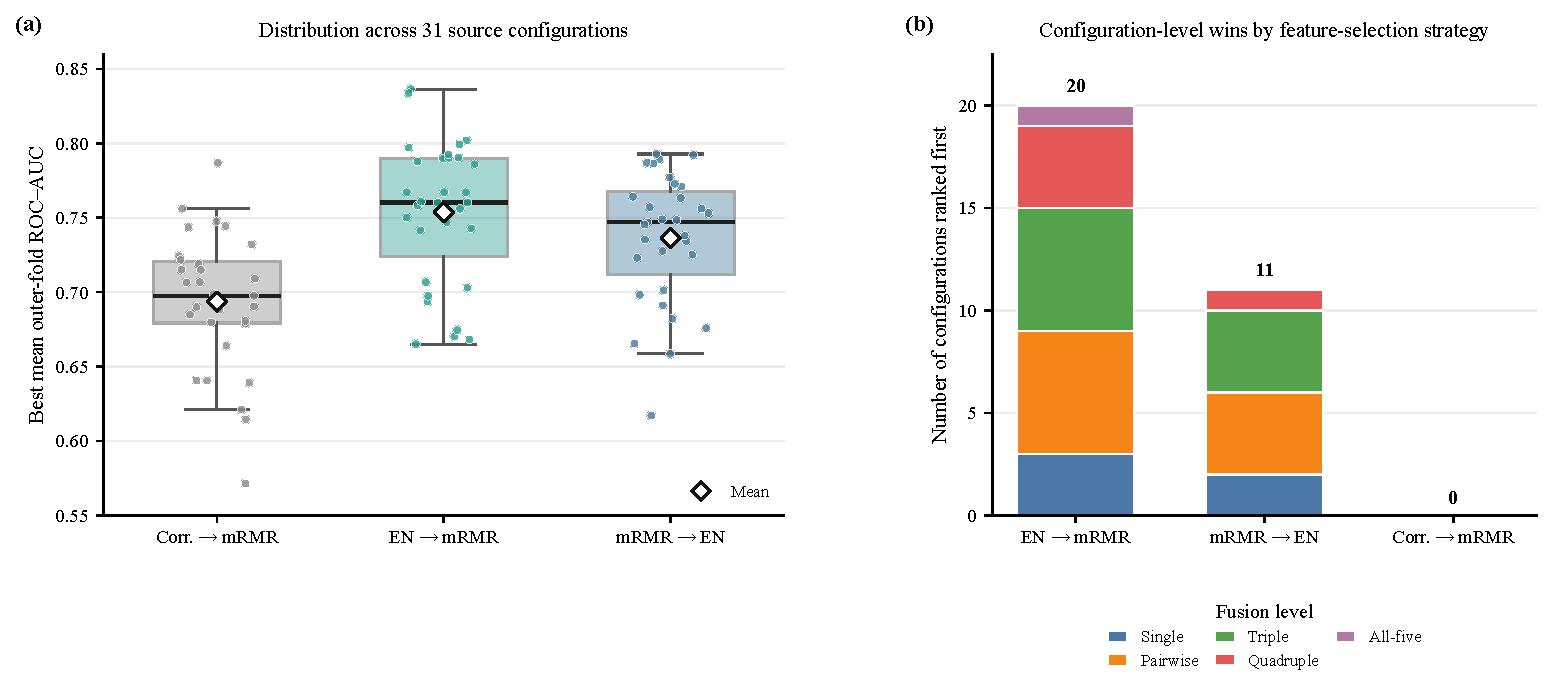
\includegraphics[width=\textwidth]
    {Figs/feature_selection_strategy_comparison.pdf}

    \caption{\textbf{Comparison of feature-selection strategies across
    the 31 source configurations.}
    (a) Distribution of the best mean outer-fold ROC-AUC obtained for
    each strategy. Points represent source configurations, boxes show
    the interquartile range, horizontal lines indicate medians, and
    white diamonds indicate means.
    (b) Number of configurations in which each strategy achieved the
    highest mean ROC-AUC, separated by feature-fusion level.
    EN, Elastic Net; mRMR, minimum redundancy maximum relevance.}
    \label{fig:feature_selection_comparison}
\end{figure*}

Elastic Net followed by mRMR produced the strongest overall results.
Its mean and median ROC-AUC values were 0.754 and 0.760, compared with
0.736 and 0.747 for mRMR followed by Elastic Net, and 0.694 and 0.698
for correlation filtering followed by mRMR.

Elastic Net followed by mRMR ranked first in 20 of the 31 source
configurations, while mRMR followed by Elastic Net ranked first in 11.
Correlation filtering followed by mRMR did not produce the
highest-ranked result for any configuration.

The advantage of Elastic Net followed by mRMR was also observed across
most fusion levels. It ranked first for three of five single-source,
six of ten pairwise, six of ten triple-source, four of five
quadruple-source, and the complete five-source configuration.

The highest ROC-AUC obtained with Elastic Net followed by mRMR was
0.836 for ADC--Post1--Pre. The corresponding maximum values for mRMR
followed by Elastic Net and correlation filtering followed by mRMR
were 0.793 and 0.787, respectively.


\subsection{Effect of SMOTE on Classification Performance}
\label{subsec:smote_results}

The effect of SMOTE was evaluated across all 31 source configurations.
For each configuration, the best SMOTE and best no-SMOTE pipelines were
identified after comparison of the three feature-selection strategies
and ten classifiers.

The difference between the two conditions was calculated as

\begin{equation}
\Delta\mathrm{AUC}_{d}
=
\mathrm{AUC}_{d,\mathrm{SMOTE}}
-
\mathrm{AUC}_{d,\mathrm{no\text{-}SMOTE}}.
\label{eq:smote_auc_difference}
\end{equation}



\begin{figure*}[htbp]
    \centering
    
\includegraphics[width=0.82\textwidth]
    {Figs/smote_effect_across_31_configurations.pdf}

    \caption{\textbf{Effect of SMOTE across the 31 source
    configurations.}
    (a) Difference in mean outer-fold ROC-AUC between the best SMOTE
    and no-SMOTE pipelines for each configuration.
    Positive values favour SMOTE and negative values favour no-SMOTE.
    (b) Number of configuration-level wins for each condition at every
    fusion level.}
    \label{fig:smote_effect_comparison}
\end{figure*}


Positive values indicate better performance with SMOTE, while negative
values indicate better performance without SMOTE.


SMOTE produced the higher mean outer-fold ROC-AUC in 19 of the 31
configurations, while no-SMOTE performed better in 12. However, the
overall difference was small. The average of the best SMOTE results
was 0.760 compared with 0.757 without SMOTE, giving an average
difference of only \(+0.003\).

For 26 of the 31 configurations, the absolute difference between the
two conditions was below 0.01 ROC-AUC. The largest improvement with
SMOTE occurred for Post1--Post2--Pre, increasing from 0.728 to 0.753
(\(+0.025\)). The largest decrease occurred for ADC--Post1--Pre,
where performance changed from 0.836 without SMOTE to 0.823 with
SMOTE (\(-0.013\)).

SMOTE performed better in four of five single-source configurations,
five of ten pairwise configurations, five of ten triple-source
configurations, and all five quadruple-source configurations. The
no-SMOTE condition performed better for the complete five-source
dataset.

Overall, the effect of SMOTE was small and depended on the source
configuration. It was therefore kept as an optional experimental
condition rather than applied to all datasets.


\subsection{Comparison of Machine-Learning Classifiers}
\label{subsec:classifier_results}


\begin{figure*}[htbp]
    \centering
    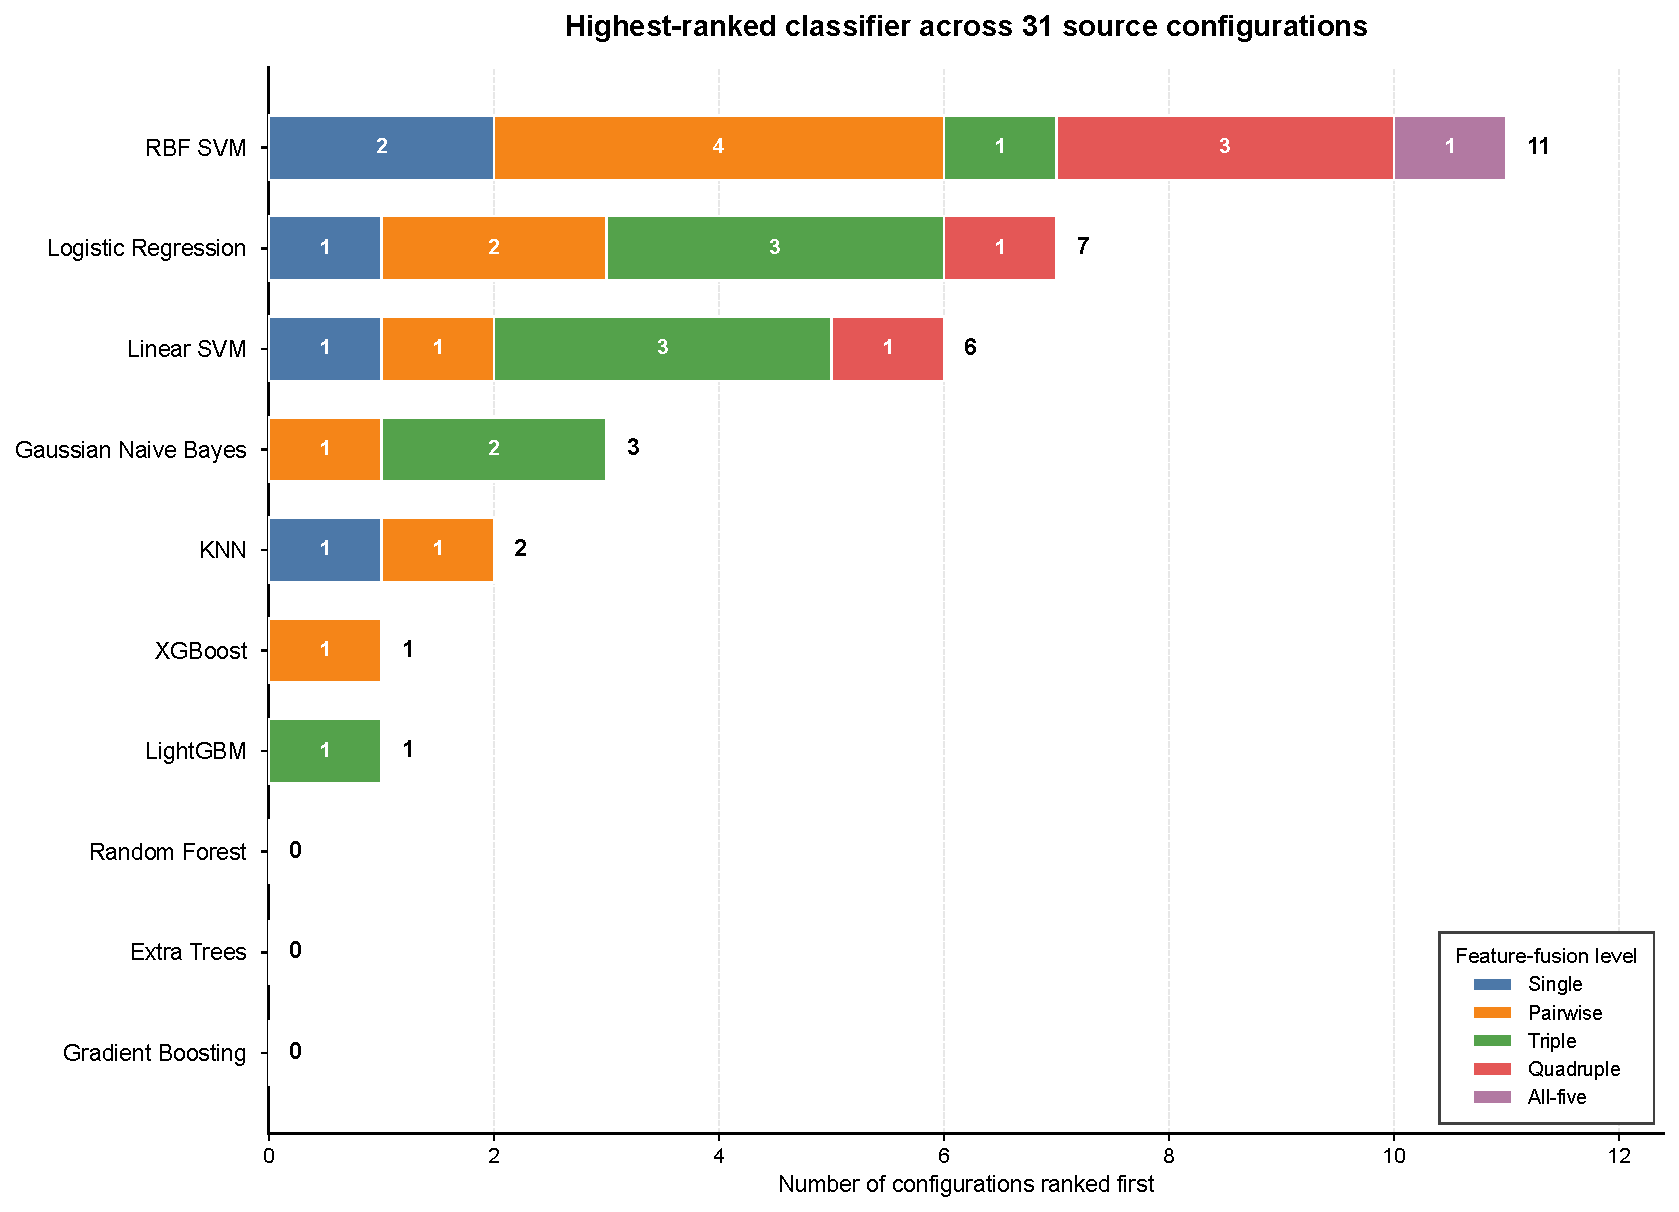
\includegraphics[width=0.82\textwidth]
    {Figs/classifier_win_counts_across_31_configurations.pdf}

    \caption{\textbf{Classifier frequency among the highest-ranked
    pipelines across the 31 source configurations.}
    Horizontal stacked bars show the number of configuration-level
    selections contributed by each feature-fusion level. Classifiers
    with no wins are retained to show all ten evaluated models.
    KNN, K-Nearest Neighbours; SVM, support vector machine.}
    \label{fig:classifier_win_counts}
\end{figure*}

Classifier selection was examined across the 31 highest-ranked
configuration-level pipelines. For each source configuration, only the
classifier belonging to the pipeline with the highest mean outer-fold
ROC-AUC was counted.



RBF SVM was the most frequently selected classifier, appearing in 11
of the 31 highest-ranked pipelines (35.5\%). Logistic Regression was
selected seven times (22.6\%), and linear SVM six times (19.4\%).
Together, the two SVM variants accounted for 17 of the 31 winning
pipelines.

Gaussian Naive Bayes was selected in three configurations,
K-Nearest Neighbours in two, and XGBoost and LightGBM once each.
Random Forest, Extra Trees, and Gradient Boosting were not selected as
the highest-ranked classifier for any source configuration.

Classifier preferences also varied with fusion level. RBF SVM was most
common among pairwise and quadruple-source configurations, while
Logistic Regression and linear SVM were more frequent among the
triple-source configurations. RBF SVM was also selected for the
complete five-source dataset.

These counts describe how often each classifier appeared in the best
pipeline for a source configuration. They do not represent the average
performance of each classifier across all experimental conditions.










\subsection{Detailed Performance of the Highest-Ranked Model}
\label{subsec:best_model_results}

The highest-ranked configuration was ADC--Post1--Pre. Its pipeline used
Elastic Net followed by mRMR, Auto-\(k\), no SMOTE, and a linear SVM.

Figure~\ref{fig:best_model_oof_performance} shows the pooled
out-of-fold performance of this model. All predictions were generated
for outer-test patients who were not used during the corresponding
model-development stage.

\begin{figure*}[htbp]
    \centering
    
\includegraphics[width=\textwidth]
    {Figs/best_overall_model_oof_performance.pdf}

    \caption{\textbf{Detailed out-of-fold performance of the
    highest-ranked pipeline.}
    The model used ADC, Post1, and Pre features with Elastic Net
    followed by mRMR, Auto-\(k\), no SMOTE, and a linear SVM.
    (a) Pooled ROC curve.
    (b) Pooled precision--recall curve.
    (c) Confusion matrix at the predefined threshold of 0.5.
    (d) Probability-calibration curve.
    All results were calculated from pooled predictions across the
    five patient-aware outer-test folds.
    AUC, area under the curve; mRMR, minimum redundancy maximum
    relevance; SVM, support vector machine.}
    \label{fig:best_model_oof_performance}
\end{figure*}

The model achieved a mean outer-fold ROC-AUC of
\(0.836 \pm 0.088\) and a pooled ROC-AUC of 0.799. Mean and pooled
PR-AUC were 0.879 and 0.832, respectively.

At the fixed classification threshold of 0.5, 81 of 113 ROIs were
classified correctly, giving a pooled accuracy of 0.717. The confusion
matrix contained 34 true negatives, 16 false positives, 16 false
negatives, and 47 true positives.

The corresponding sensitivity and precision were both 0.746,
specificity was 0.680, balanced accuracy was 0.713, and the F1-score
was 0.746. Cohen's kappa was 0.426, and the pooled Brier score was
0.183.

Auto-\(k\) selected an average of 9.6 features across the five outer
folds, with feature counts ranging from 4 to 18. In total, 28 different
features were selected in at least one fold. No feature appeared in all
five folds, while the most frequently selected feature appeared in four.

Feature-selection stability and SHAP-based interpretation are reported
in Section~\ref{subsec:interpretability_results}.









\subsection{Feature-Selection Stability and Model Interpretation}
\label{subsec:interpretability_results}

Feature-selection stability and SHAP interpretation were examined for
the highest-ranked ADC--Post1--Pre pipeline, which used Elastic Net
followed by mRMR, Auto-\(k\), no SMOTE, and a linear SVM.

Feature selection was performed independently in each of the five
outer folds. Auto-\(k\) selected an average of 9.6 features per fold,
and 28 different features were selected at least once. Features
selected in at least two folds were considered recurrent.

Thirteen features met this criterion
(Figure~\ref{fig:best_model_stability_shap}(a)). No feature was
selected in all five folds. The most stable feature was the ADC
intensity-histogram median, which appeared in four folds. Five other
features appeared in three folds, while the remaining recurrent
features appeared in two. All recurrent features originated from ADC
or Post1; no Pre-derived feature was selected in at least two folds.

\begin{figure*}[htbp]
    \centering
    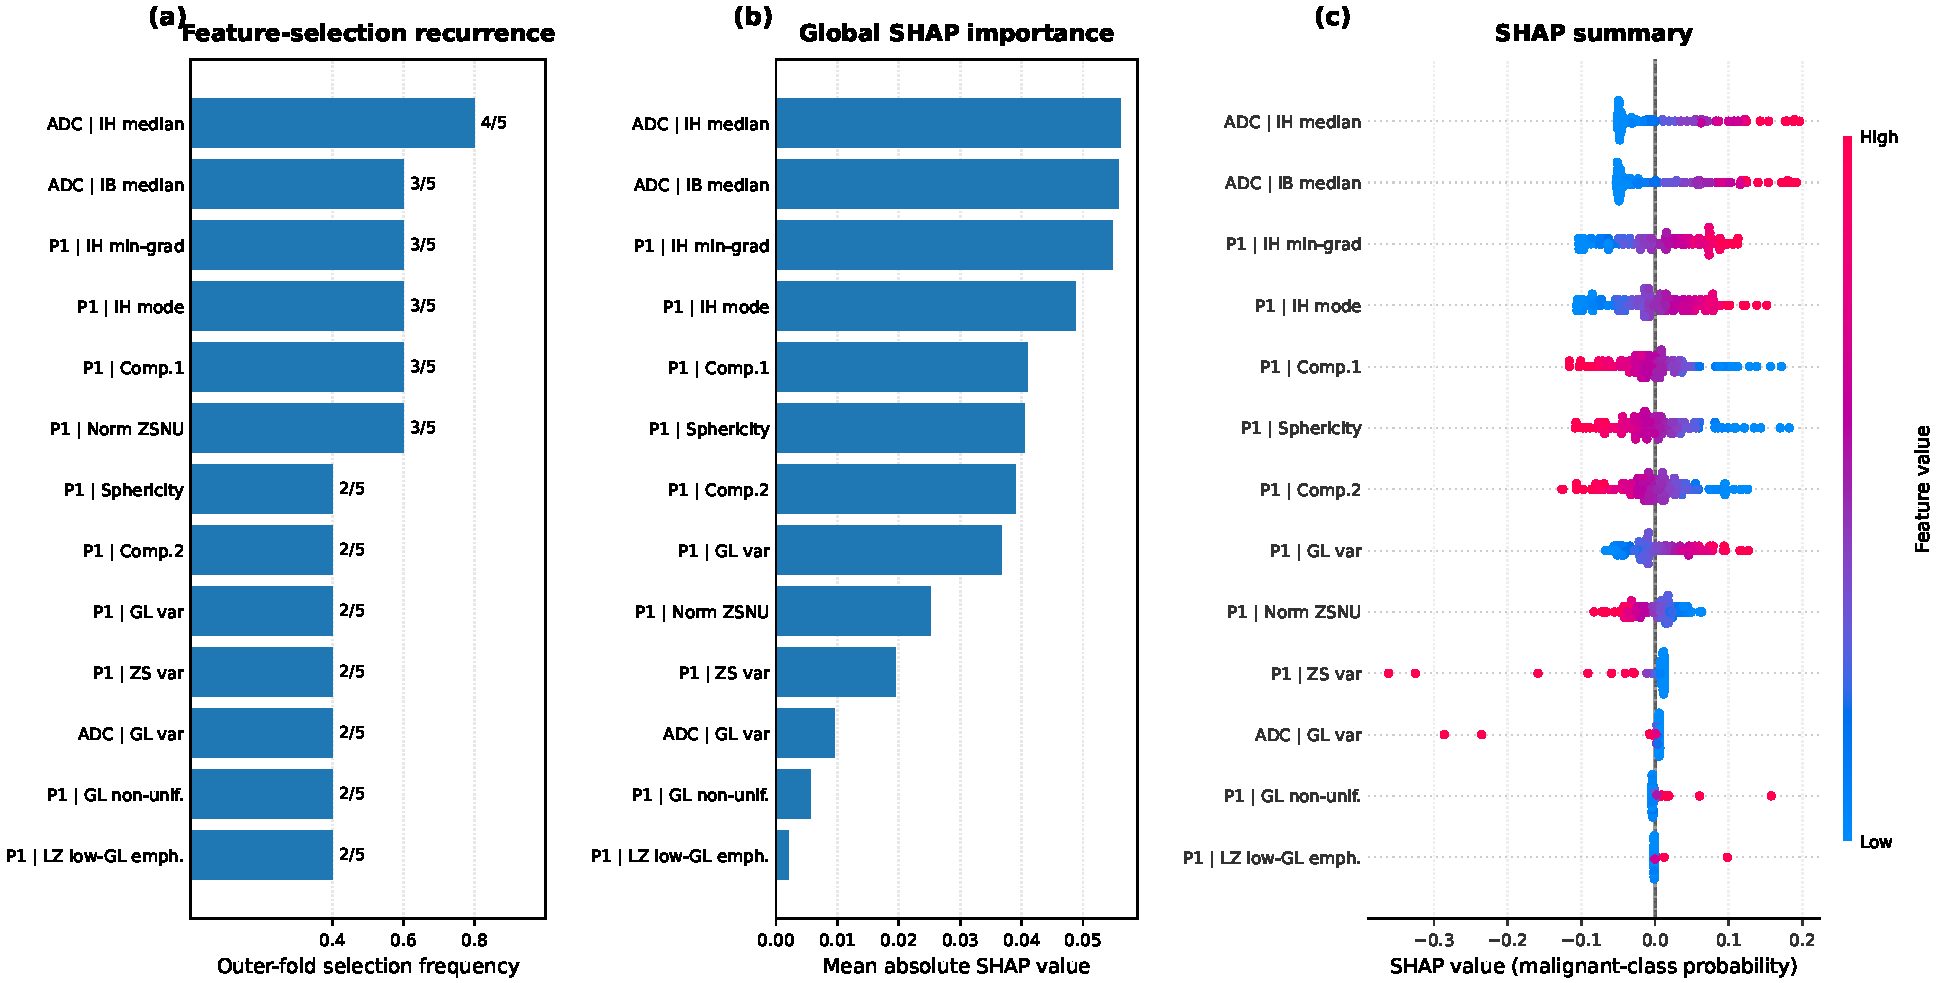
\includegraphics[width=\textwidth]
    {Figs/best_model_feature_stability_and_shap.pdf}

    \caption{\textbf{Feature-selection stability and SHAP
    interpretation of the highest-ranked ADC--Post1--Pre pipeline.}
    (a) Selection frequency of features retained in at least two of
    the five outer folds.
    (b) Global feature importance measured by mean absolute SHAP value.
    (c) SHAP summary plot showing the magnitude and direction of
    feature contributions across ROIs. Positive SHAP values move the
    model output toward the malignant class, while negative values move
    it toward the benign class. Feature names were shortened for
    readability.
    P1, Post1; IH, intensity histogram; IB, intensity based;
    Comp., compactness; GL, grey level; ZS, zone size; ZSNU,
    zone-size non-uniformity; mRMR, minimum redundancy maximum
    relevance; SHAP, Shapley Additive Explanations; SVM, support
    vector machine.
    The full-cohort model was used only for interpretation; predictive
    performance was estimated from patient-aware out-of-fold
    predictions.}
    \label{fig:best_model_stability_shap}
\end{figure*}

For SHAP analysis, a separate linear SVM was refitted using the
recurrent features and the complete cohort. This model was used only
for interpretation and did not contribute to the reported performance
estimates.

As shown in Figure~\ref{fig:best_model_stability_shap}(b), the ADC
intensity-histogram median and ADC intensity-based median had the
largest mean absolute SHAP values. Two Post1 intensity-histogram
features followed them, while several Post1 morphological and texture
features also contributed to the model.

The SHAP summary plot
(Figure~\ref{fig:best_model_stability_shap}(c)) shows the direction of
these effects. Higher values of the leading ADC intensity features and
the main Post1 intensity-histogram features were generally associated
with higher malignant-class model outputs. In contrast, higher values
of some Post1 morphological features, including Compactness and
Sphericity, were more often associated with lower malignant-class
outputs.

Feature-selection frequency and SHAP importance describe different
properties. Selection frequency measures how consistently a feature
was retained across patient groups, whereas SHAP measures its influence
within the fitted interpretation model. SHAP results were therefore
used to explain model behaviour and not as evidence of causal or
biological effects.



























\section{Discussion}
\label{sec:discussion}

\subsection{Principal Findings}
\label{subsec:discussion_principal_findings}

This study compared all 31 possible combinations of five MRI-derived
radiomic feature sources using the same patient-aware machine-learning
framework. The main finding was that combining all available sources
did not give the best result. Instead, the highest performance was
obtained from a selected triple-source combination.

The best pipeline used ADC, Post1, and Pre features with Elastic Net
followed by mRMR, Auto-\(k\), no SMOTE, and a linear SVM. It achieved
a mean outer-fold ROC-AUC of \(0.836 \pm 0.088\). A second
triple-source combination, ADC--Post2--T2, achieved a very similar
result of \(0.834 \pm 0.045\). In comparison, the complete five-source
model achieved a lower mean ROC-AUC of \(0.747 \pm 0.117\).

Feature-selection order also influenced performance. Elastic Net
followed by mRMR ranked first in 20 of the 31 source configurations,
while mRMR followed by Elastic Net ranked first in 11. Correlation
filtering followed by mRMR did not produce a configuration-level
winner.

The overall effect of SMOTE was small. Although SMOTE produced a
higher result in more configurations, most differences were less than
0.01 ROC-AUC, and the best overall pipeline did not use SMOTE.

Classifier performance also depended on the source configuration.
RBF SVM was selected most frequently, followed by Logistic Regression
and linear SVM. However, the highest overall performance was obtained
with linear SVM.

The best model achieved a pooled ROC-AUC of 0.799, pooled PR-AUC of
0.832, balanced accuracy of 0.713, and F1-score of 0.746. It selected
an average of 9.6 features per outer fold, although the exact selected
features varied across folds.

Overall, the findings suggest that selective multi-source integration
was more effective than complete feature concatenation and that model
performance depended on the combined effects of source selection,
feature selection, SMOTE, and classifier choice.


\subsection{Effect of Multi-Source Feature Integration}
\label{subsec:discussion_feature_integration}

Combining feature sources improved performance in some cases, but the
improvement depended on which sources were combined.

The best mean ROC-AUC increased from 0.790 for a single-source dataset
to 0.799 for a pairwise combination and 0.836 for a triple-source
combination. However, performance decreased to 0.802 for the best
quadruple-source configuration and 0.747 when all five sources were
combined.

One possible explanation is the rapid increase in dimensionality.
Single-source datasets contained about 145 predictors, compared with
approximately 435 for triple-source datasets, 580 for quadruple-source
datasets, and 724 for the complete five-source dataset. In contrast,
the number of independent patients remained approximately 48.

Therefore, adding sources increased the number of candidate predictors
without increasing the amount of independent training data. This can
make feature selection more difficult and increase sensitivity to the
patients included in each training fold.

The results also showed that the identity of the combined sources was
more important than the number of sources alone. Different pairwise
and triple-source combinations produced substantially different
results despite having similar numbers of features and observations.

ADC appeared in many of the highest-ranked combinations. However, this
does not prove that ADC alone was responsible for the improvement,
because performance depended on its combination with other sources,
the selected features, and the classifier.

These results support evaluating different source combinations
directly rather than assuming that using all available sources will
produce the best model.


\subsection{Influence of Feature-Selection Strategy}
\label{subsec:discussion_feature_selection}

Feature-selection strategy had a clear effect on model performance.
Elastic Net followed by mRMR produced the highest result in 20 of the
31 source configurations, while mRMR followed by Elastic Net ranked
first in the remaining 11.

Although these two strategies used the same methods, changing their
order changed the intermediate candidate feature space and therefore
the final selected subset.

In the Elastic-Net--mRMR pipeline, Elastic Net first performed a
supervised and regularised reduction of the full feature space. mRMR
then selected a smaller subset while considering both relevance and
redundancy. This ordering produced the strongest average performance
in the present study.

The reverse order remained competitive, showing that no single
feature-selection sequence was optimal for every source configuration.

Correlation filtering followed by mRMR performed less favourably.
Removing highly correlated predictors before supervised multivariable
selection may remove variables that could still provide useful
information when combined with other features.

Overall, the results show that feature selection should be considered
part of the complete modelling pipeline rather than as an independent
preprocessing step.


\subsection{Effect of SMOTE and Class Imbalance}
\label{subsec:discussion_smote}

SMOTE did not consistently improve classification performance. It
produced a higher mean ROC-AUC in 19 of the 31 source configurations,
while no-SMOTE performed better in 12. However, the average difference
between the two conditions was only about 0.003 ROC-AUC.

For 26 of the 31 configurations, the absolute difference was below
0.01. This indicates that the overall effect of SMOTE on discrimination
was small.

The limited effect may partly reflect the relatively mild class
imbalance in the datasets. For example, the complete five-source
dataset contained 50 benign and 63 malignant ROIs.

SMOTE can still change threshold-dependent measures because it modifies
the training distribution and therefore the fitted decision boundary.
This may improve balanced accuracy, specificity, or precision even when
ROC-AUC changes very little.

The two highest-ranked triple-source models and the complete
five-source winner were obtained without SMOTE. In contrast, SMOTE was
selected for several other successful pipelines, including all five
quadruple-source winners.

These results suggest that SMOTE should be tested as an optional part
of the modelling pipeline rather than applied automatically.


\subsection{Classifier Performance and Model Complexity}
\label{subsec:discussion_classifiers}

No classifier was optimal for every source configuration. RBF SVM was
selected most often, appearing in 11 of the 31 highest-ranked
pipelines. Logistic Regression was selected seven times and linear SVM
six times.

The strongest overall model nevertheless used a linear SVM. This shows
that the classifier selected most frequently was not necessarily the
classifier producing the highest individual result.

The strong performance of linear SVM and Logistic Regression suggests
that relatively simple regularised models remained competitive after
feature selection. The selected feature subsets may have provided
enough separation for linear decision boundaries to perform well.

Tree-based ensemble models were less frequently selected. XGBoost and
LightGBM each appeared once, while Random Forest, Extra Trees, and
Gradient Boosting did not produce any configuration-level winner.

This should not be interpreted as evidence that tree-based methods are
generally unsuitable. Their performance may have been affected by the
small number of independent patients and the limited hyperparameter
search budget.

Each Optuna study used only ten trials. This provided a consistent
comparison across the large experimental grid but may have been more
restrictive for models with larger hyperparameter spaces.

Overall, classifier choice depended strongly on the source
representation and selected features, with regularised linear and
kernel-based models providing the most frequent high-performing
solutions.


\subsection{Feature Stability and Model Interpretation}
\label{subsec:discussion_interpretability}

The feature-stability analysis showed that strong predictive
performance did not require exactly the same features to be selected
in every training fold.

The best ADC--Post1--Pre pipeline selected an average of 9.6 features
per outer fold. Across all five folds, 28 different features were
selected at least once, 13 appeared in at least two folds, and none was
selected in every fold.

This variability may result from the high-dimensional feature space
and the relatively small number of independent patients. Several
correlated or similarly informative predictors may provide comparable
information, allowing different feature subsets to support similar
classification performance.

The recurrent feature set contained features from ADC and Post1. No
Pre-derived feature appeared in at least two folds. However, this does
not mean that Pre was uninformative, because the best-performing source
configuration included Pre and different Pre features may have
contributed in individual folds.

SHAP analysis showed that the interpretation model relied most strongly
on two ADC intensity features, together with several Post1 intensity,
morphological, and texture features.

Feature-selection frequency and SHAP importance should be interpreted
differently. Selection frequency measures how consistently a feature
is retained across training samples, whereas SHAP describes its
influence within a fitted model.

The SHAP model was refitted using the complete cohort only for
interpretation. Therefore, the SHAP results describe the behaviour of
the fitted model and should not be considered independent evidence of
feature importance or biological causality.


\subsection{Strengths and Limitations}
\label{subsec:discussion_strengths_limitations}

A major strength of this study was the use of patient-aware nested
cross-validation. All ROIs from the same patient remained in the same
fold, reducing the risk of patient-level data leakage. Preprocessing,
feature selection, Auto-\(k\), SMOTE, and hyperparameter optimisation
were also restricted to the appropriate training data.

Another strength was the systematic evaluation of all 31 source
combinations using the same modelling framework. This allowed
single-source and multi-source representations to be compared under
consistent conditions.

Several performance measures were also reported in addition to the
primary mean outer-fold ROC-AUC, including pooled ROC-AUC, PR-AUC,
threshold-dependent metrics, calibration, feature stability, and SHAP
interpretation.

The main limitation was the small number of independent patients.
Although more than 100 ROIs were available, the datasets represented
approximately 48 patients. The effective sample size was therefore much
smaller than the number of observations.

The study also did not include an independent external test cohort.
Nested cross-validation reduces optimisation bias, but the best model
was still selected from many candidate pipelines evaluated within the
same cohort. External validation is therefore required.

Hyperparameter optimisation was limited to ten Optuna trials per study.
This was necessary to keep the large computational experiment
manageable but did not provide an exhaustive search, particularly for
more complex classifiers.

Another limitation was the use of direct feature concatenation for
multi-source integration. More advanced fusion methods may produce
different results.

Finally, the selected features were not highly stable across outer
folds, and SHAP interpretation was based on a separate full-cohort
refit. These results should therefore be viewed as model explanations
rather than evidence of a fixed radiomic signature or causal
relationship.

Overall, the present framework provides a controlled comparison of
candidate modelling strategies, but the results require confirmation
in independent data.


\subsection{Future Work and Generalisability}
\label{subsec:discussion_future_work}

The most important next step is external validation of the
ADC--Post1--Pre pipeline in an independent cohort. The complete
pipeline, including preprocessing, feature selection, Auto-\(k\), and
classifier fitting, should be evaluated rather than testing only the
final classifier.

Larger datasets with more independent patients would also improve the
precision of performance estimates and provide a stronger assessment
of feature-selection stability.

Future studies should investigate whether selective source integration
continues to outperform complete concatenation in larger cohorts.
Alternative fusion approaches, such as source-specific feature
selection, prediction-level fusion, or representation-learning
methods, could also be compared with direct concatenation.

A larger hyperparameter-optimisation budget may be useful for the most
promising classifiers identified in this study, particularly models
with larger search spaces.

Future work could also optimise the classification threshold using
training data only and evaluate the selected threshold on independent
patients. This would allow sensitivity and specificity to be adjusted
for a predefined application.

Feature stability and SHAP interpretation should also be repeated in
external datasets to determine whether the same sources, feature
families, and individual predictors remain important.

Overall, the ADC--Post1--Pre pipeline represents the strongest
candidate identified in the present study. However, larger and
independent cohorts are required before its predictive performance,
selected features, and model interpretation can be considered
generalisable.










\section{Conclusion}
\label{sec:conclusion}

This study compared all 31 possible combinations of five MRI-derived
radiomic feature sources using a patient-aware nested cross-validation
framework. The results showed that combining more feature sources did
not always improve classification performance.

The best result was obtained with the ADC--Post1--Pre combination using
Elastic Net followed by mRMR, Auto-\(k\), no SMOTE, and a linear SVM.
This pipeline achieved a mean outer-fold ROC-AUC of
\(0.836 \pm 0.088\) and a pooled ROC-AUC of 0.799.

Performance also depended on the feature-selection strategy, SMOTE
condition, and classifier, showing that these components should be
evaluated together as part of the complete modelling pipeline.
Feature-selection stability analysis further showed that good
predictive performance could be achieved even when the exact selected
features changed across patient folds.

Overall, selective multi-source integration provided better results
than complete feature concatenation in this dataset. However, the
selected ADC--Post1--Pre pipeline was developed using a limited cohort,
and validation in larger independent datasets is required before its
performance and selected features can be considered generalisable.
\end{document}
